\NeedsTeXFormat{LaTeX2e}
\documentclass[10pt,a4]{scrartcl}

\usepackage{tabularx,graphicx,a4,listings,wrapfig,subfigure}

\ifx\pdfoutput\undefined
  % We're not running pdftex
  % european (better) fonts -- does not look good with pdflatex
  \usepackage[T1]{fontenc}
  \newcommand{\href}[2]{#2\\{\hspace*{5mm}\scriptsize <#1>}\\}
\else
  \pdfcompresslevel=9
  \def\pdfBorderAttrs{/Border [0 0 0] } % No border around Links
  \usepackage{hyperref}
\fi

\title{Equalizer Programming Guide\\
  {\footnotesize\sffamily\mdseries
    \htmladdnormallink{http://www.equalizergraphics.com/documents/Developer/ProgrammingGuide.pdf}
    {http://www.equalizergraphics.com/documents/ProgrammingGuide.pdf}}
}
\author{Stefan Eilemann\\{\footnotesize Eyescale Software GmbH}
}
\date{
  \vspace{4cm}
  \begin{figure}[ht]
    \hspace{-4.5cm}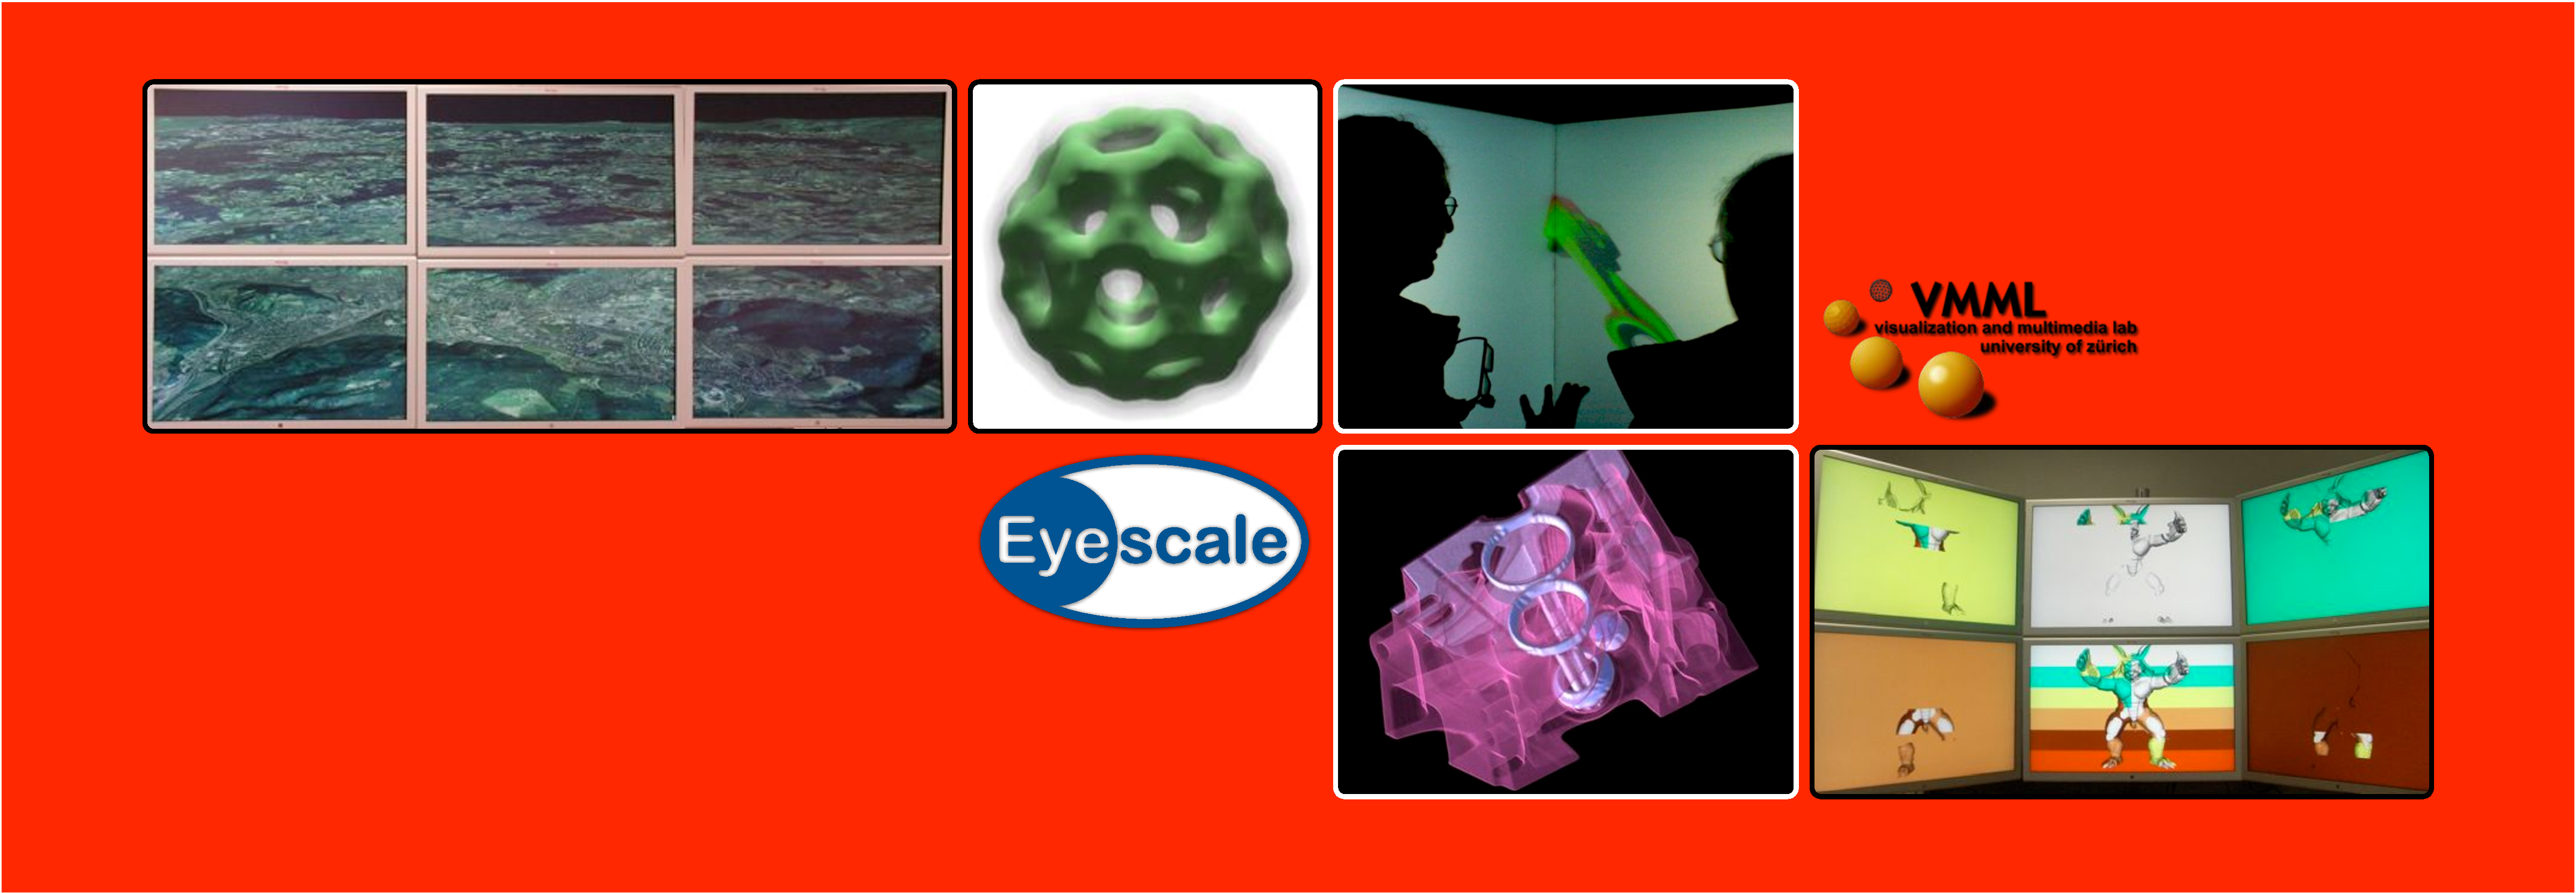
\includegraphics[width=22cm]{images/teaser.pdf}
  \end{figure}
  \vspace{1cm}
  \textbf{DRAFT}\\[\medskipamount]
  Version 0.9.1 for Equalizer v0.4\\[\medskipamount]
  \today
}

\newcommand{\tm}{\texttrademark~}
\newcommand{\rc}{\raise 1ex\hbox{{\tiny\textregistered}}~}
\newcommand{\fig}[1]{Figure~\ref{#1}}
\newcommand{\sref}[1]{Section~\ref{#1}}
\newcommand{\link}[1]{\htmladdnormallink{#1}{#1}}

% suppress  single floating lines on top (widow) and bottom(club)
%  10000 is infinity
%  tradeoff: maybe underfull vboxes
\clubpenalty=10000
\widowpenalty=10000 

\begin{document}

\maketitle
\vfill
\lstset{language=C++}

\thispagestyle{empty}

%\abstract{
%  Equalizer is a project to develop software to simplify the creation of
%  scalable graphics applications and to improve the usability of
%  multipipe visualization systems.
%}


\clearpage
\tableofcontents
\thispagestyle{empty}
\vfill{\center\begin{tabularx}{\textwidth}{|l|l|X|}
    \hline
    \bf Rev & \bf Date     & \bf Changes \\
    \hline
    0.9.1   & Oct 8, 2007  & review pass\\
    0.9     & Oct 7, 2007  & add eqHello, draft assembly in eVolve\\
    0.8     & Sep 28, 2007 & add head tracking, finish channel,
                             proof-reading pass\\
    0.7     & Sep 21, 2007 & start channel and image compositing,
                             add event handling, move to new eqPly
                             code base\\
    0.6     & Sep 14, 2007 & add pipe, window and object manager\\
    0.5     & Sep 3,  2007 & add config and partly pipe\\
    0.4     & Aug 31, 2007 & add distributed objects\\
    0.3     & Aug 26, 2007 & add application and render client\\
    0.2     & Aug 20, 2007 & add main function\\
    0.1     & Aug 19, 2007 & outline the basic concepts\\
    \hline
  \end{tabularx}}
\thispagestyle{empty}
\clearpage

\pagenumbering{arabic}



\section{Introduction}

Equalizer provides a framework for the development of parallel
OpenGL\texttrademark\ applications. Equalizer-based applications can run
a single shared-memory system with multiple graphics cards (GPU's) or on
graphics clusters. This Programming Guide introduces the programming
interface using the \textsf{eqPly} example shipped with Equalizer as a
guideline.

Any questions related to Equalizer programming and this Programming
Guide should be directed to the \textsf{eq-dev} mailing
list\footnote{see \link{http://www.equalizergraphics.com/lists.html}}.

Equalizer is the next evolution of generic parallel programming
interfaces for visualization applications using OpenGL. Existing
solutions, such as SGI's OpenGL Multipipe\texttrademark\ SDK, VRCO's
Cavelib\texttrademark\ and VRJuggler, implement a subset of concepts
similar to Equalizer. In other areas, e.g., tracking device support,
they provide more functionality.

Equalizer implements the minimum necessary layer to build parallel and
scalable OpenGL applications. The programmer structures the application
so that the OpenGL rendering can be executed in parallel, potentially
using multiple processes for cluster-based execution. Equalizer provides
the domain-specific parallel rendering know-how and abstracts
configuration, threading, synchronization, windowing and event
handling. It is a `GLUT on steroids', providing parallel and distributed
execution, scalable rendering features and fully customizable event
handling.

\section{Getting Started}


\subsection{Compiling and running \textsf{eqPly}}

It is recommended to have a compiled version of Equalizer and the
examples when working with this Programming Guide. The Quickstart
Guide\footnote{\link{http://www.equalizergraphics.com/documents/EqualizerGuide.html}}
should be executed once to get familar with the capabilities of the
\textsf{eqPly} example.

Compiling Equalizer is as simple as running \textsf{make} on Linux or
building the Equalizer Visual Studio 2005 solution on Windows. On Mac OS
X 10.4 (Tiger), some prerequisites have to be installed before running
\textsf{make}, as explained in \textsf{README.Darwin}. Mac OS X 10.5
Leopard does have all the prerequisites installed by default.


\subsection{Equalizer Processes}

\begin{wrapfigure}{r}{.4\textwidth}
  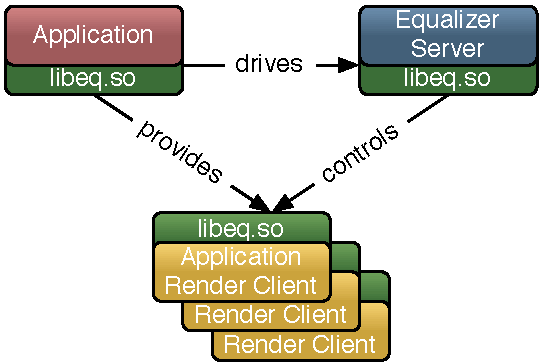
\includegraphics[width=.4\textwidth]{images/processes.pdf}
  {\caption{\small\label{fProcesses}Equalizer Processes}}
\end{wrapfigure}
All functionality of Equalizer is accessed through the Equalizer client
library, which implements all functionality discussed in this
document. The client library provides communication between the Equalizer
processes.

\subsubsection{Server}

An Equalizer server is responsible for managing one visualization
system, i.e., a shared memory system or graphics cluster. Currently it
is only useful for running one application at a time, but it will be
extended to support multiple applications concurrently and efficiently
on one system. The server controls and potentially launches the
application's rendering clients.

\subsubsection{Application}

The application connects to an Equalizer server, which chooses a
configuration for the application. Furthermore, the application also
provides its render client, which will be controlled by the server. The
application reacts on events, updates its database and controls the
rendering.

\subsubsection{Render Clients}

The render client implements --obviously-- the rendering part of an
application. Its execution is passive, that is, it has no main loop and
is completely driven by rendering tasks received from the server. The
tasks are executed by calling the appropriate task methods (see
\sref{ssTaskMethods}) in the correct thread and context.

The application might be a rendering client, in which case it can also
contribute to the rendering. If it does not implement any render
client-related code it is reduced to be the application's `master'
process without any OpenGL windows.

The rendering client can be the same executable as the application, as
it is the case with \textsf{eqPly}. When it is started as a render client,
the Equalizer initialization routine does not return and takes over the
control by calling the render client task methods. Complex real-world
applications often implement a separate, light-weight rendering client.



\section{Hello, World!}

\begin{wrapfigure}{r}{.6\textwidth}
  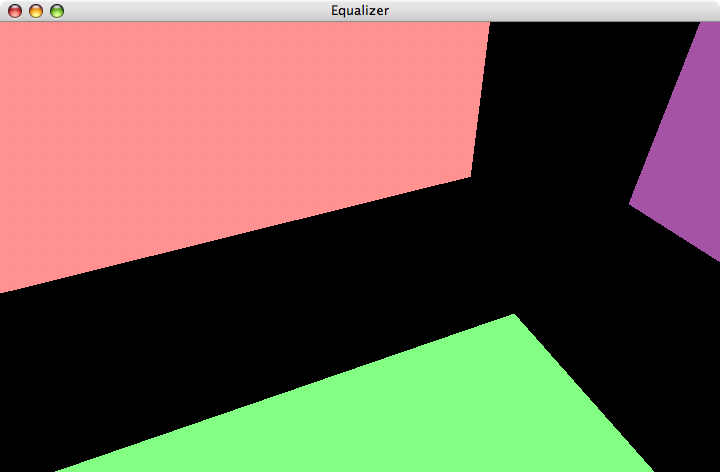
\includegraphics[width=.6\textwidth]{images/eqHello.png}
  {\caption{\small\label{fHello}Hello, World!}}
\end{wrapfigure}

The \textsf{eqHello} example is a minimal example to illustrate the
basic principle of an Equalizer application: The application developer
has to implement the rendering method \textsf{Channel::frameDraw},
similar to the \textsf{glutDisplayFunc} in GLUT applications. It can be
run as a stand-alone application from the command line.

The \textsf{eqHello} redraw function renders six rotating, colored quads
around the origin, where the viewer is usually positioned. The Equalizer
\textsf{frameDraw} meth\-od is used as a convience function to setup the
frustum and other OpenGL state. After setting up some additional
lighting parameter, \textsf{eqHello} rotates the scene and render the
quads using immediate mode:

{\footnotesize\begin{lstlisting}
void Channel::frameDraw( const uint32_t spin )
{
    // setup OpenGL State
    eq::Channel::frameDraw( spin );
    
    const float lightPos[] = { 0.0f, 0.0f, 1.0f, 0.0f };
    glLightfv( GL_LIGHT0, GL_POSITION, lightPos );

    const float lightAmbient[] = { 0.2f, 0.2f, 0.2f, 1.0f };
    glLightfv( GL_LIGHT0, GL_AMBIENT, lightAmbient );

    // rotate scene around the origin
    glRotatef( static_cast< float >( spin ) * 0.5f, 1.0f, 0.5f, 0.25f );

    // render six axis-aligned colored quads around the origin
    [...]
}
\end{lstlisting}}

The \textsf{eqHello} main function sets up the communication with the
server, initializes and drives the rendering. The details of this setup
are explained in \sref{sEqPly}.



\section{The Programming Interface}

Equalizer uses a C++ programming interface. The API is minimally
invasive, that is, Equalizer imposes only the minimal, natural execution
framework upon the application. It does not provide a scene graph or
does interfere in any other way with the application's rendering
code. The restructuring work needed for Equalizer is needed anyway in
order to parallelize the application for rendering.

Methods called by the application have the form \textsf{verb[Noun]},
whereas methods called by Equalizer (`Task Methods') have the form
\textsf{nounVerb}. For example the application calls
\textsf{Config::startFrame} to render a new frame, which causes --among
other things-- \textsf{Node::frameStart} to be called in all active
render clients.


\subsection{\label{ssTaskMethods}Task Methods}

The application subclasses Equalizer objects and overrides virtual
functions to implement certain functionality, e.g., the application's
OpenGL rendering in \textsf{eq::Chan\-nel::frameDraw}. These task
methods are in concept similar to C function callbacks. The
\textsf{eqPly} section will discuss the most important task methods. A
full list can be found on the website\footnote{see
  \link{http://www.equalizergraphics.com/documents/design/taskMethods.html}}.

\if 0
\subsection{Thread Safety}

Using threading correctly in OpenGL-based applications is easy with
Equalizer. Equalizer creates one rendering thread for each graphics
card. All task methods for a pipe, and therefore all OpenGL commands,
are executed from this thread. This threading model is the OpenGL
`threading model', which maintains one current context for each
thread. It is difficult, if not impossible, to render from different
threads to the same context.

The rendering threads concurrently render the application's data
base. The data base should be accessed in a read-only fashion during
rendering, as it is the case with all modern scene graphs.

The rendering threads run asynchronously to the application's main
thread. Depending on the configuration's latency, the fall $n$ frames
behind the last frame finished by the application thread.

TBD support and explain per-node frame sync.
\fi

\subsection{\label{sResource}The Resource Tree}

The rendering resources are represented in a hierarchical tree structure
which corresponds to the physical and logical resources found in a 3D
rendering environment. 

\begin{figure}[ht!]\center
  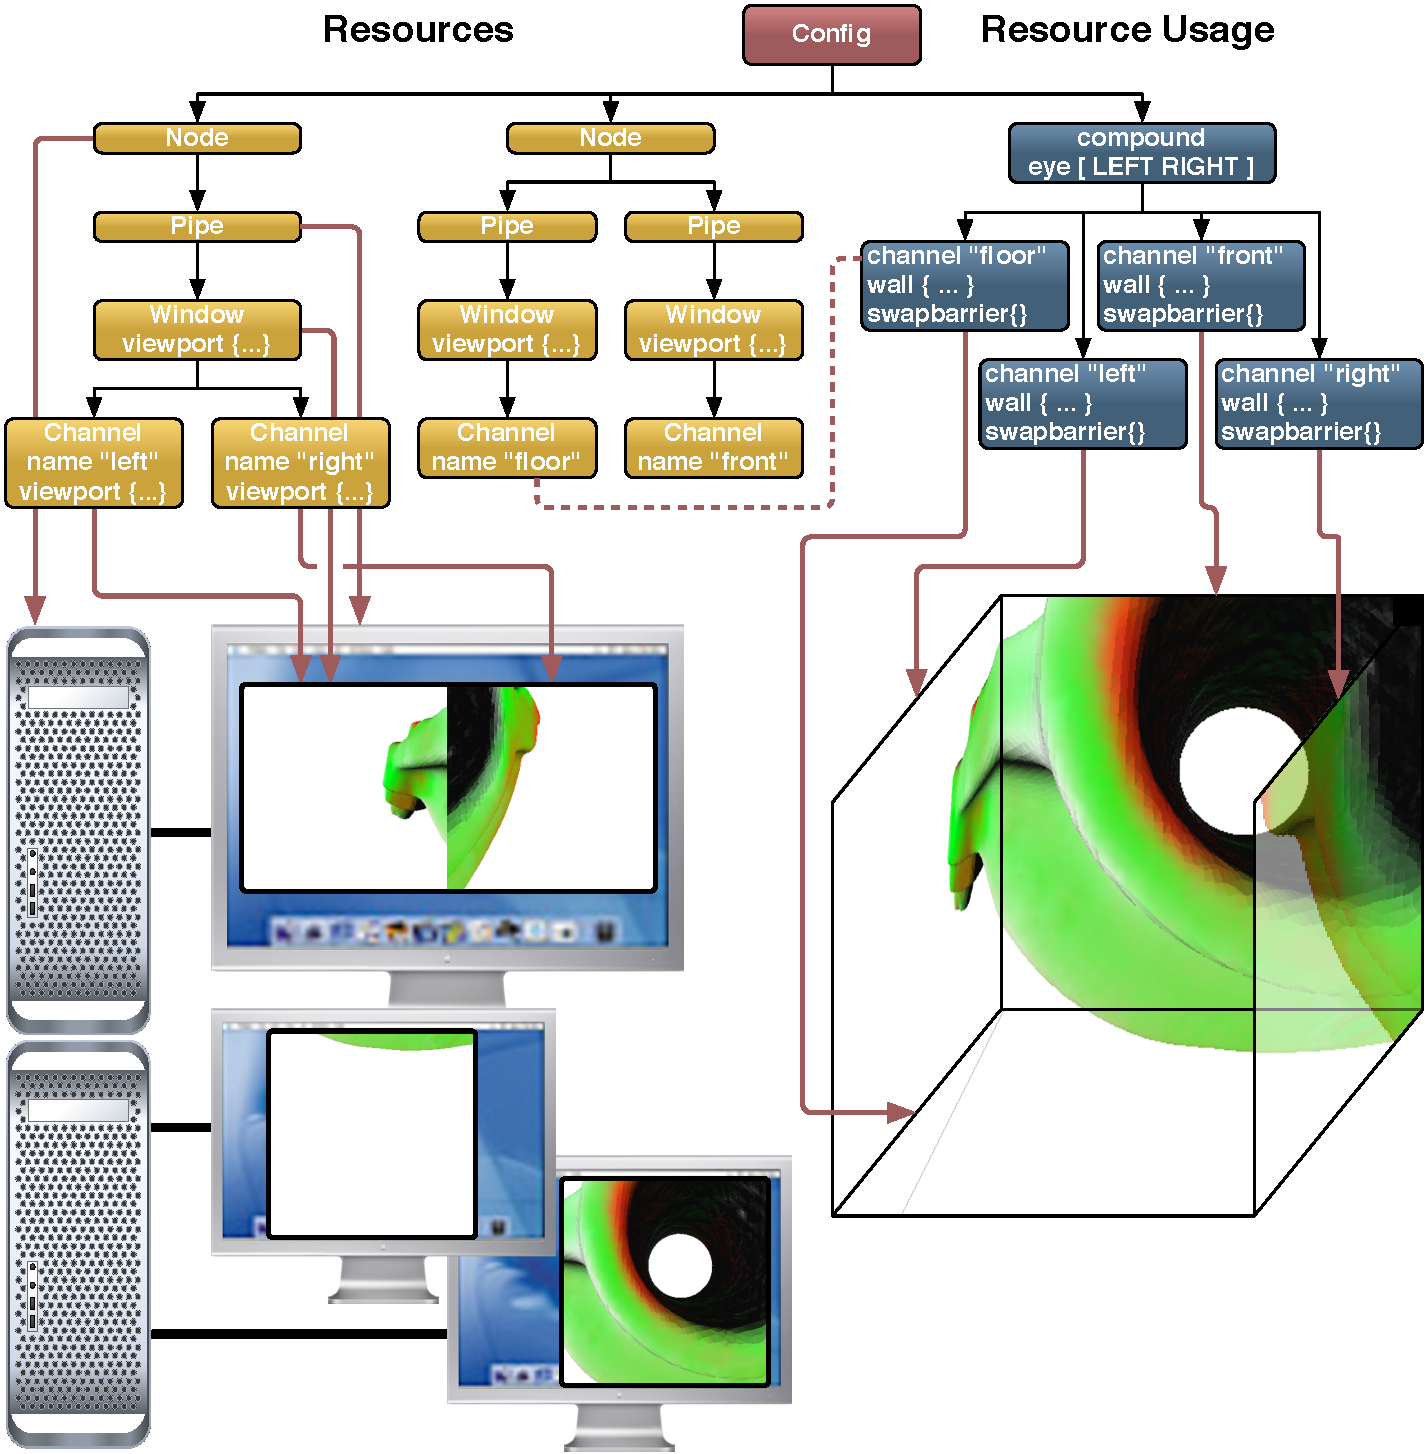
\includegraphics[width=.9\textwidth]{images/cave.pdf}
  {\caption{\small\label{fConfig}An example configuration}}
\end{figure}

\fig{fConfig} shows one example configuration for a four-side
CAVE\texttrademark, running on two machines (node) using three graphics
cards (pipe) with one window each to render to the four output channels
connected to the projectors for each of the walls. The compound
description is only used by the server to compute the rendering
tasks. The application is not aware of compounds, and does not need to
concern itself with the parallel rendering logics of a configuration.

For testing and development purposes it is possible to use multiple
instances for one resource, e.g., to run multiple render client nodes on
one computer. For deployment one node and pipe should be used for each
computer and graphics card, respectively.

\subsubsection{Configuration}

The root of the resource tree is the \textsf{eq::Config}, which
represents the current configuration of the application. The
configuration is the session in which all render clients are
registered. The config instance on a given node currently only holds the
local node, not all nodes of the configuration.

\subsubsection{Node}

An \textsf{eq::Node} is the representation of a single computer in the
system. One operating system process of the render client will be used
for each node. Each configuration might also use an application node, in
which case the application process is also used for rendering. All
node-specific task methods are executed from the main application
thread.

\subsubsection{Pipe}

The \textsf{eq::Pipe} is the abstraction of a graphics card (GPU). In
the current implementation it is also one operating system thread,
unless the pipe's thread hint is set to \textsf{false}. All pipe, window
and channel task methods are executed from the pipe thread pipes or from
the main application thread for non-threaded pipes\footnote{see
  \link{http://www.equalizergraphics.com/documents/design/nonthreaded.html}}.

Further versions of Equalizer might introduce threaded windows, where
all window-related task methods are executed in a separate operating
system thread.

\subsubsection{Window}

An \textsf{eq::Window} holds a drawable and OpenGL context. The
drawable can be an on-screen window or an off-screen PBuffer or
FBO\footnote{off-screen drawables are not yet implemented, but can be
  created by the application and used with Equalizer}. The window holds
window-system-specific handles to the drawable and context, e.g., an X11
window \textsf{XID} and \textsf{GLXContext} for the glX window system.

\subsubsection{Channel}

The \textsf{eq::Channel} is the abstraction of an OpenGL viewport within
its parent window. It is the entity executing the actual rendering. The
channel's viewport might be overwritten when it is rendering for another
channel.


\subsection{Compounds}

How the rendering resources are to be used is configured using a
compound tree. Although the API does not currently expose compounds, the
basic design behind compounds is explained here to increase the
understanding of the architecture behind Equalizer.

Each compound has a channel, which it uses to execute the rendering
tasks. One channel might be used by multiple compounds. Unused channels
are not instantiated. The rendering tasks for the channels are computed
by the server and send to the appropriate render clients.

\begin{wrapfigure}{r}{.6\textwidth}
  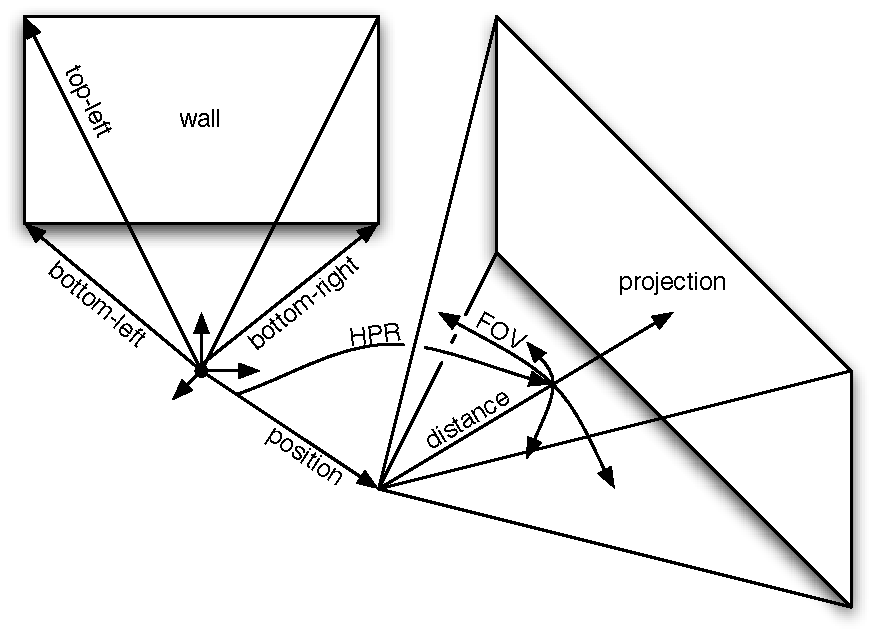
\includegraphics[width=.6\textwidth]{images/frustra.pdf}
  {\caption{\small\label{fFrustra}Frustrum descriptions}}
\end{wrapfigure}
The channels of the leaf compounds (source channels) in the compound
tree execute the rendering for the top-most compound's channel
(destination channel). The top-most compound with a channel defines the
2D pixel viewport rendered by all leaf compounds. The destination
channel and pixel viewport can not be overridden.

Compounds have a frustum description, which is inherited to the
children. The frustum can be overridden by children, but this is rarely
used since there is no use case for this behaviour. 

The frustrum can be specified as a wall, which is completely defined by
the bottom-left, bottom-right and top-left coordinates relative to the
origin, or as a projection, which is defined by the position and
head-pitch-roll orientation of the projector, as well as the horizontal
and vertical field-of-view and distance of the projection
wall. \fig{fFrustra} illustrates the wall and projection frustum
parameters.

Compounds have attributes which configure the decomposition of the
destination's channel viewport, frustum and database. A
\textsf{viewport} decomposes the destination channel and frustum in
screen space. A \textsf{range} tells the application to render a part of
its database, and an eye pass can selectively render different stereo
passes.

Compounds have output and input frames which configure the recomposition
of the resulting pixels from the source compound channels. An output
frame connects to an input frame of the same name, which transports the
selected frame buffer data from the output channel to the input
channel. This composition process is extensively described in
\sref{sCompositing}.

More information on the configuration of compounds can be found on the
Equalizer website\footnote{see
  \link{http://www.equalizergraphics.com/documents/design/compounds.html}}.



\section{\label{sEqPly}The eqPly polygonal renderer}

The \textsf{eqPly} example is shipped with the Equalizer distribution
and serves as a reference implementation of an Equalizer-based
application of medium complexity. Its focus is not on rendering features
or visual quality, but it is used as a show case for the integration of
most of the Equalizer features.

In this section the source code of \textsf{eqPly} is discussed in
detail, and relevant design decision, caveat and remarks are raised.

All classes in the example are in the \textsf{eqPly} namespace to avoid
type name ambiguities, in particular for the \textsf{Window} class which
is frequently used as a type in the global namespace by windowing
systems. \fig{fUml} shows the most important Equalizer classes and how
they are subclassed by the \textsf{eqPly} example.

The derived classes fall into two categories: The subclassed rendering
entities as discussed in \sref{sResource}, and two classes for
distributing data. For each of the rendering entities, its function and
typical usage will be discussed. The distributed data classes illustrate
the typical usage of static and dynamic, frame-specific data.

\begin{figure}[ht!]\center
  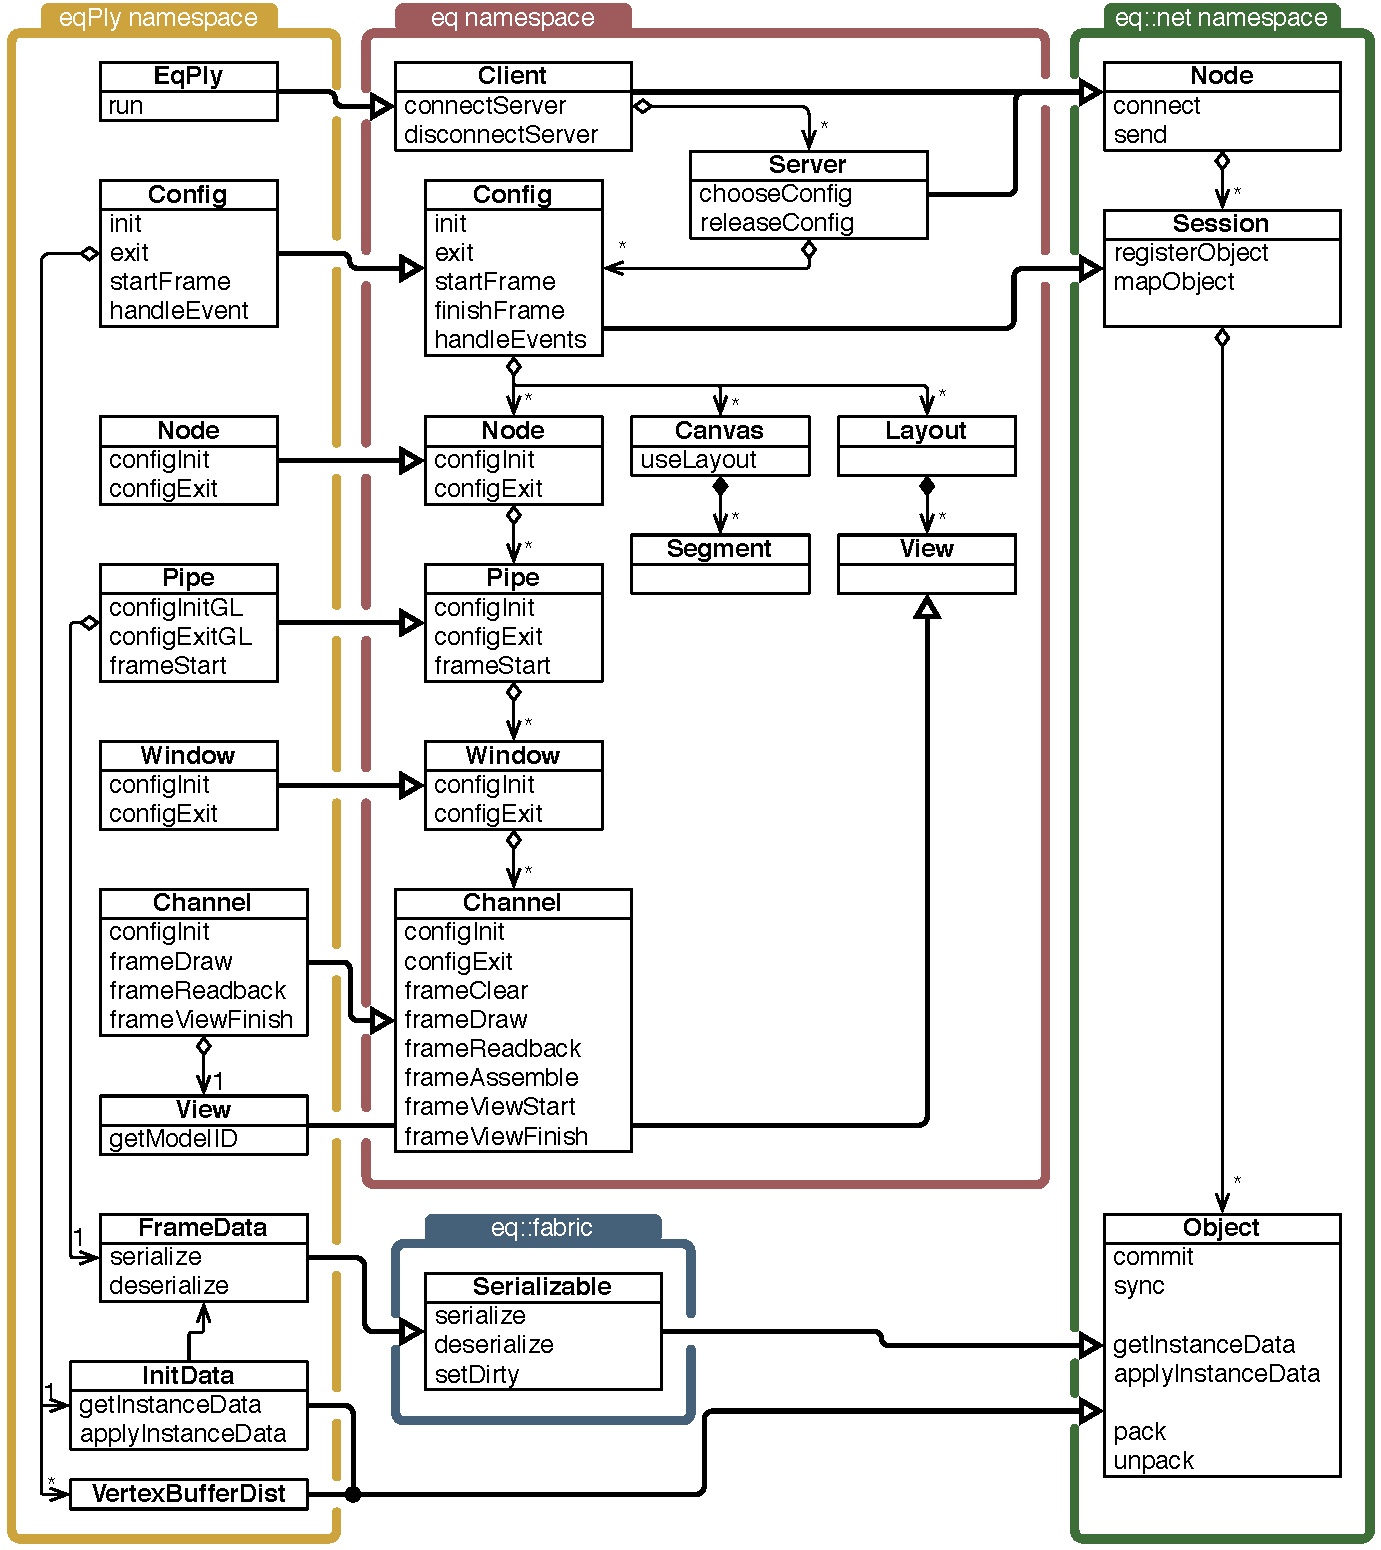
\includegraphics[width=\textwidth]{images/uml}
  {\caption{\small\label{fUml}UML diagram of significant Equalizer and
      eqPly classes and task methods.}}
\end{figure}


\subsection{The main Function}

The main function starts off with parsing the command line into the
\textsf{LocalInitData} data structure, part of which will be distributed
to all render client nodes. The actual command line parsing is done by
the \textsf{LocalInitData} class and will be discussed in
\sref{sInitData}:

{\footnotesize\begin{lstlisting}
int main( int argc, char** argv )
{
    // 1. parse arguments
    eqPly::LocalInitData initData;
    initData.parseArguments( argc, argv );
\end{lstlisting}}

The second step is to initialize the Equalizer library. The
initialization function of Equalizer also parses the command line, which
is used to set certain default values based on Equalizer-specific
options\footnote{Equalizer-specific options always start with -\,-eq-},
e.g., the default server address. Furthermore, a \textsf{NodeFactory} is
provided. The \textsf{EQERROR} macro, and its counterparts
\textsf{EQWARN}, \textsf{EQINFO} and \textsf{EQVERB} allow selective
debugging outputs with various logging levels:

{\footnotesize\begin{lstlisting}
    // 2. Equalizer initialization
    NodeFactory nodeFactory;
    if( !eq::init( argc, argv, &nodeFactory ))
    {
        EQERROR << "Equalizer init failed" << endl;
        return EXIT_FAILURE;
    }
\end{lstlisting}}%>>

The node factory is used by Equalizer to create the object instances for
the rendering entities. Each of the classes inherits from the same type
provided by Equalizer in the \textsf{eq} namespace. The provided
\textsf{eq::NodeFactory} base class instantiates a 'plain' Equalizer
object, thus making it possible to selectively subclass individual
entity types, as it is done by \textsf{eqHello}. For each rendering
resource used in the configuration, one C++ object will be created:

{\footnotesize\begin{lstlisting}
class NodeFactory : public eq::NodeFactory
{
public:
    virtual eq::Config*  createConfig()  { return new eqPly::Config; }
    virtual eq::Node*    createNode()    { return new eqPly::Node; }
    virtual eq::Pipe*    createPipe()    { return new eqPly::Pipe; }
    virtual eq::Window*  createWindow()  { return new eqPly::Window; }
    virtual eq::Channel* createChannel() { return new eqPly::Channel; }
};
\end{lstlisting}}

The third step is to create an instance of the application and to
initialize it locally. The application is an \textsf{eq::Client}, which
in turn is an \textsf{eqNet::Node}. The underlying network distribution
in Equalizer is a peer-to-peer network structure of
\textsf{eqNet::Node}s. The application programmer rarely is aware of the
classes in the \textsf{eqNet} namespace, but both the
\textsf{eq::Client} and the server are \textsf{eqNet::Node}s. The local
initialization of nodes creates a local listening socket, so that the
node, and therefore the \textsf{eq::Client} can communicate over the
network with other nodes, such as the server and the rendering clients.

{\footnotesize\begin{lstlisting}
    // 3. initialization of local client node
    RefPtr< eqPly::Application > client = new eqPly::Application( initData );
    if( !client->initLocal( argc, argv ))
    {
        EQERROR << "Can't init client" << endl;
        eq::exit();
        return EXIT_FAILURE;
    }
\end{lstlisting}}%>>

Finally everything is set up to run the \textsf{eqPly} application:

{\footnotesize\begin{lstlisting}
    // 4. run client
    const int ret = client->run();
\end{lstlisting}}

After it has finished, the application and \textsf{eqPly} is
de-initialized and the \textsf{main} function returns:

{\footnotesize\begin{lstlisting}
    // 5. cleanup and exit
    client->exitLocal();
    client = 0;

    eq::exit();
    return ret;
}
\end{lstlisting}}


\subsection{Application}

In the case of \textsf{eqPly} the application is also the render
client. The \textsf{eqPly} executable has three run-time behaviours:

\begin{enumerate}
  \item \textbf{Application}: The executable started by the user, which
    is the controlling entity in the rendering session.
  \item \textbf{Auto-launched render client}: The typical render client,
    started by the server. The server starts the executable with special
    parameters, which cause \textsf{Client::initLocal} to never
    return. During exit, the server terminates the process. By default,
    the server starts render client using \textsf{ssh}.
  \item \textbf{Resident render client}: Manually pre-started render
    client, listening on a specified port for server commands. This mode
    is selected using the command-line option \textsf{--eq-client} and
    potentially \textsf{--eq-listen} and \textsf{-r}\footnote{see \link{http://www.equalizergraphics.com/documents/design/residentNodes.html}}.
\end{enumerate}

\subsubsection{Main Loop}

The application's main loop starts by connecting the application to an
Equalizer server. The command line parameter \textsf{--eq-server}
explicitly specifies a server address. If no server was specified,
\textsf{Client::connectServer} try first to connect to a server on the
local machine using the default port 4242. If that fails, it will create
a server running within the applications process with a default
1-channel configuration\footnote{see
  \link{http://www.equalizergraphics.com/documents/design/standalone.html}}.

{\footnotesize\begin{lstlisting}
int Application::run()
{
    // 1. connect to server
    RefPtr<eq::Server> server = new eq::Server;
    if( !connectServer( server ))
    {
        EQERROR << "Can't open server" << endl;
        return EXIT_FAILURE;
    }
\end{lstlisting}}%>>

The second step is to ask the server for a configuration. The
\textsf{ConfigParams} are a placeholder for later Equalizer
implementations to provide additional hints and information to the
server for choosing a configuration. The configuration chosen by the
server is created locally using
\textsf{NodeFactory::createConfig}. Therefore it is of type
\textsf{eqPly::Config}, but the return value is \textsf{eq::Config},
making cast necessary:

{\footnotesize\begin{lstlisting}
    // 2. choose config
    eq::ConfigParams configParams;
    Config* config = static_cast<Config*>(server->chooseConfig( configParams ));

    if( !config )
    {
        EQERROR << "No matching config on server" << endl;
        disconnectServer( server );
        return EXIT_FAILURE;
    }
\end{lstlisting}}%>>

Finally it is time to initialize the configuration. For statistics, the
time for this operation is measures and printed. During initialization
the server launches and connects all render client nodes, and calls the
appropriate initialization task methods, as explained in later
sections. \textsf{Config::init} does return after all nodes, pipes,
windows and channels are initialized. It returns \textsf{true} only if
all initialization task methods were successful.

The \textsf{EQLOG} macro allows topic-specific logging. The numeric
topic values are specified in the respective \textsf{log.h} header
files, and logging for various topics is enables using the environment
variable \textsf{EQ\_LOG\_TOPICS}:

{\footnotesize\begin{lstlisting}
    // 3. init config
    eqBase::Clock clock;

    config->setInitData( _initData );
    if( !config->init( ))
    {
        EQERROR << "Config initialization failed: " 
                << config->getErrorMessage() << endl;
        server->releaseConfig( config );
        disconnectServer( server );
        return EXIT_FAILURE;
    }

    EQLOG( eq::LOG_CUSTOM ) << "Config init took " << clock.getTimef() << " ms"
                            << endl;
\end{lstlisting}}%>>

When the configuration was successfully initialized, the main rendering
loop is executed. The main loop runs until either the user exits the
configuration or a maximum number of frames has been rendered, specified
as a command-line argument. The latter is useful for benchmarks. The
\textsf{Clock} is reused for measuring the overall performance. A new
frame is started using \textsf{Config::startFrame} and a frame is
finished using \textsf{Config::finishFrame}.

When the frame is started, the server computes all rendering tasks and
sends them to the appropriate render client nodes. The render client
nodes dispatch the tasks to the correct node or pipe thread, were they
are executed in the order they arrive.

\begin{wrapfigure}{r}{.6\textwidth}
  \subfigure[]{\label{fSync}
    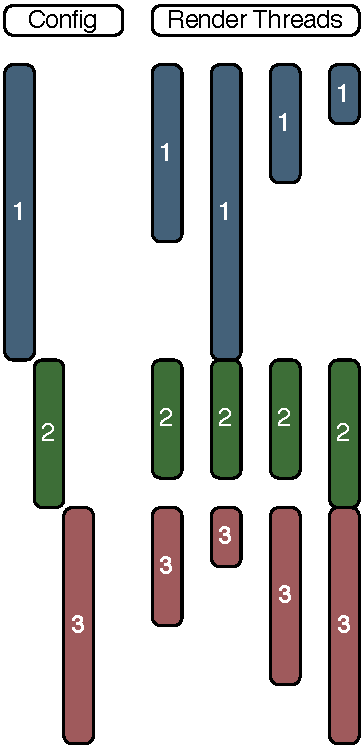
\includegraphics[width=.25\textwidth]{images/sync}}\hfil
  \subfigure[]{\label{fAsync}
    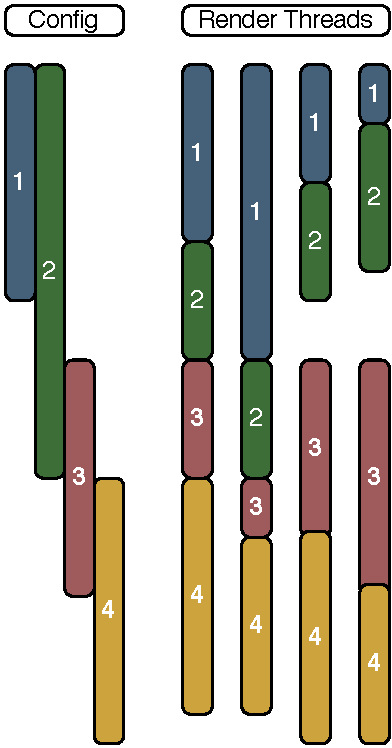
\includegraphics[width=.25\textwidth]{images/async}}%
  {\caption{\small\label{fSyncAsync}Synchronous and asynchronous execution}}
\end{wrapfigure}
\textsf{Config::finishFrame} synchronizes on the completion of the frame
\textsf{current - latency}. The latency is specified in the
configuration file, and allows several outstanding frames. This allows
overlapped execution in the node and pipe threads and minimizes idle
times. The first \textsf{nLatency Config::finishFrame} return
immediately, since they have no frame to synchronize
upon. \fig{fSyncAsync} shows the execution of (hypothetical) rendering
tasks without latency~(\fig{fSync}) and with a latency of
one~(\fig{fAsync}). 

With \textsf{eqPly} a speedup of 15\% has been observed on a five-node
rendering
cluster when using a latency of one instead of no latency\footnote{\link{http://www.equalizergraphics.com/scalability.html}}.

When the main loop is finished, \textsf{Config::finishAllFrames} catches
up with the latency. It returns after all outstanding frames have been
rendered, and is needed here to provide an accurate measurement of the
framerate:

{\footnotesize\begin{lstlisting}
    // 4. run main loop
    uint32_t maxFrames = _initData.getMaxFrames();
    
    clock.reset();
    while( config->isRunning( ) && maxFrames-- )
    {
        config->startFrame();
        // config->renderData(...);
        config->finishFrame();
    }
    const uint32_t frame = config->finishAllFrames();
    const float    time  = clock.getTimef();
    EQLOG( eq::LOG_CUSTOM ) << "Rendering took " << time << " ms (" << frame
                            << " frames @ " << ( frame / time * 1000.f)
                            << " FPS)" << endl;
\end{lstlisting}}%>>

The remainder of the application code cleans up in the reverse order of
the initialization. The config is exited, released and the connection to
the server is closed:

{\footnotesize\begin{lstlisting}
    // 5. exit config
    clock.reset();
    config->exit();
    EQLOG( eq::LOG_CUSTOM ) << "Exit took " << clock.getTimef() << " ms" <<endl;

    // 6. cleanup and exit
    server->releaseConfig( config );
    if( !disconnectServer( server ))
        EQERROR << "Client::disconnectServer failed" << endl;
    server = 0;
    return EXIT_SUCCESS;
}
\end{lstlisting}}%>>

\subsubsection{Render Clients}

In the second and third usage case of the \textsf{eqPly}, when the
executable is used as a render client, \textsf{Client::initLocal} never
returns. Therefore the application's main loop is never executed. In
order to keep the client resident, the \textsf{eqPly} example overrides
the client loop to keep it running beyond one configuration run:

{\footnotesize\begin{lstlisting}
bool Application::clientLoop()
{
    if( !_initData.isResident( )) // execute only one config run
        return eq::Client::clientLoop();

    // else execute client loops 'forever'
    while( true ) // TODO: implement SIGHUP handler to exit?
    {
        if( !eq::Client::clientLoop( ))
            return false;
        EQINFO << "One configuration run successfully executed" << endl;
    }
    return true;
}
\end{lstlisting}}%>>


\subsection{Distributed Objects}

Equalizer provides distributed objects which help implementing data
distribution in a graphics cluster. The master version of a distributed
object is registered with a \textsf{eqNet::Session}, which assigns a
session-unique identifier to the object. Other nodes can map their
instance of the object to this identifier, thus synchronizing the
object's data with the remotely registered object.

Distributed objects are created by subclassing from
\textsf{eqNet::Object}. Distributed objects can be static (immutable) or
dynamic. Dynamic objects are versioned.

The \textsf{eqPly} example has a static distributed object to provide
initial data to all rendering nodes, as well as a versioned object to
provide frame-specific data, such as the camera position, to the
rendering methods.

\subsubsection{\label{sInitData}InitData - a Static Distributed Object}

The \textsf{InitData} class holds a couple of parameters needed during
initialization. These parameters never change during one configuration
run, and are therefore static.

On the application side, the class \textsf{LocalInitData} subclasses
\textsf{InitData} to provide the command line parsing and to set the
initial values. The render nodes only instantiate the distributed part
in \textsf{InitData}

A static distributed object either has to provide a pointer and size to
its data using \textsf{setInstanceData}, or it has to implement
\textsf{getInstanceData} and \textsf{applyInstanceData}. The first
approach can be used if all distributed member variables can be outlayed
in one contiguous block of memory. The second approach is used
otherwise.

The \textsf{InitData} class contains a string of variable
length. Therefore it uses the second approach of manually serializing
and deserializing its data. The serialization is done in
\textsf{getInstanceData} and deserialization in
\textsf{applyInstanceData} by streaming all member variable to or from
the provided data streams. The data transport between nodes is
implemented in the data streams and various other Equalizer classes:

{\footnotesize\begin{lstlisting}
void InitData::getInstanceData( eqNet::DataOStream& os )
{
    os << _frameDataID << _windowSystem << _useVBOs << _useShaders << _filename;
}

void InitData::applyInstanceData( eqNet::DataIStream& is )
{
    is >> _frameDataID >> _windowSystem >> _useVBOs >> _useShaders >> _filename;

    EQASSERT( _frameDataID != EQ_ID_INVALID );
    EQINFO << "New InitData instance" << endl;
}
\end{lstlisting}}%>>

The data output and input streams perform no type checking on the data
stream. It is the application's responsibility to match the order and
types of variables during serialization and deserialization exactly.

\subsubsection{FrameData - a Versioned Distributed Object}

Versioned objects have to override \textsf{isStatic} to return false, to
indicate that they are versioned. The current implementation has the
following characteristics:
\begin{itemize}
\item Only the master instance of the object is writable, that is,
  \textsf{eqNet::Object::com\-mit} can be called to generate a new
  version.
\item Slave instance versions can only be advanced, that is,
  \textsf{eqNet::Object::sync( version )} with a version smaller than
  the current version will fail.
\end{itemize}

Upon \textsf{commit} the delta data from the previous version is sent to
all mapped slave instances. The data is queued on the remote node, and
is applied when the application calls \textsf{sync} to synchronize the
object to a new version. The \textsf{sync} method might block if a
version has not been committed or is still in transmission.

In addition to the instance data (de)serialization methods needed to map
an object, versioned objects may implement \textsf{pack} and
\textsf{unpack} to serialize or deserialize the changes since the last
version.

If the delta data happens to be layed out contiguously in memory,
\textsf{setDeltaData} might be used. The default implementation of
\textsf{pack} and \textsf{unpack} (de)serialize the delta data or the
instance data if no delta data has been specified.

The \textsf{eqPly} frame data is layed out in one anonymous structure in
memory. It also does not track changes since it is relatively small in
size and changes frequently. Therefore, the instance and delta data are
the same and set in the constructor:

{\footnotesize\begin{lstlisting}
        FrameData()
            {
                reset();
                setInstanceData( &data, sizeof( Data ));
                EQINFO << "New FrameData " << std::endl;
            }
\end{lstlisting}}%>>

\subsection{Config}

The configuration is driving the application's rendering, that is, it is
responsible for updating the data based on received events, requesting
new frames to be rendered and to provide the render clients with the
necessary data.

\subsubsection{Initialization and Exit}

The config initialization happens in parallel, that is, all config
initialization tasks are transmitted by the server at once and their
execution is synchronized later. 

The tasks are executed by the node and pipe threads in parallel. The
parent's initialization methods are always executed before any child
initialization method. This parallelization is necessary to allow a
speedy startup of the configuration on large-scale graphics clusters. On
the other hand, it means that initialization functions are called even
if the parent's initialization has failed.

\begin{wrapfigure}{r}{.6\textwidth}
  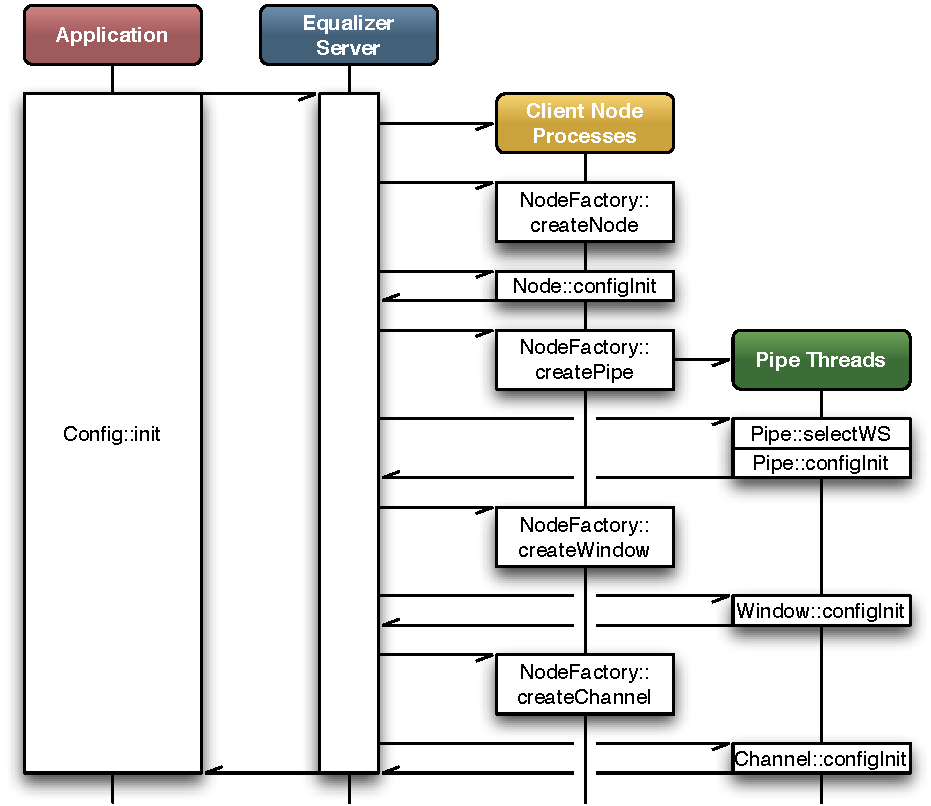
\includegraphics[width=.6\textwidth]{images/configInit.pdf}
  {\caption{\small\label{fConfigInit}Config Initialization Sequence}}
\end{wrapfigure}
The \textsf{eqPly::Config} class holds the master versions of the
initialization and frame data. Both objects are registered with the
\textsf{eq::Config}, which is the \textsf{eqNet::Session} used for
rendering. Equalizer takes care of the session setup and exit in
\textsf{Client::choose\-Config} and \textsf{Client::releaseConfig},
respectively.

The frame data is registered first, since its identifier is transmitted
using the initialization data. The initialization data is registered
afterwards so that it can transmit the frame data's identifier. The
identifier of the initialization data is transmitted to the render
client nodes using the \textsf{initID} parameter of
\textsf{eq::Config::init}. Equalizer will pass this identifier to all
\textsf{configInit} calls of the respective objects:

{\footnotesize\begin{lstlisting}
bool Config::init()
{
    // init distributed objects
    _frameData.data.color = _initData.useColor();
    registerObject( &_frameData );
    _initData.setFrameDataID( _frameData.getID( ));

    registerObject( &_initData );

    // init config
    _running = eq::Config::init( _initData.getID( ));
    if( !_running )
        return false;
\end{lstlisting}}

If the configuration was initialized correctly, the configuration tries
to set up a tracking device for head tracking. Equalizer does not
provide extensive support for tracking device, as this is an orthogonal
problem to parallel rendering. Tracking device support has been solved
already by a number of implementations\footnote{VRCO Trackd, VRPN,
  etc.}, which can easily be integrated with Equalizer. The example code
in \textsf{eqPly} is one reference implementation for the integration of
such a tracking library:

{\footnotesize\begin{lstlisting}
    // init tracker
    if( !_initData.getTrackerPort().empty( ))
    {
        if( !_tracker.init( _initData.getTrackerPort() ))
            EQWARN << "Failed to initialise tracker" << endl;
        else
        {
            // Set up position of tracking system in world space
            // Note: this depends on the physical installation.
            vmml::Matrix4f m( vmml::Matrix4f::IDENTITY );
            m.scale( 1.f, 1.f, -1.f );
            //m.x = .5;
            _tracker.setWorldToEmitter( m );

            m = vmml::Matrix4f::IDENTITY;
            m.rotateZ( -M_PI_2 );
            _tracker.setSensorToObject( m );
            EQLOG( eq::LOG_CUSTOM ) << "Tracker initialised" << endl;
        }
    }

    return true;
}
\end{lstlisting}}%>>

The exit of the configuration stops the render clients by calling
\textsf{eq::Config::exit}, and then deregisters the initialization and
frame data objects with the session:

{\footnotesize\begin{lstlisting}
bool Config::exit()
{
    _running = false;
    const bool ret = eq::Config::exit();

    _initData.setFrameDataID( EQ_ID_INVALID );
    deregisterObject( &_initData );
    deregisterObject( &_frameData );

    return ret;
}
\end{lstlisting}}

\subsubsection{Frame Control}

The rendering frames are issued by the application. The \textsf{Config}
only overrides \textsf{startFrame} in order to update its data before
forwarding the start frame request to the \textsf{eq::Config}.

If a tracker is used, the current head position and orientation is
retrieved and given to Equalizer, which uses the head matrix together
with the wall or projection description to compute the view
frustra\footnote{see
  \link{http://www.equalizergraphics.com/documents/design/immersive.html}}.

The camera position is updated and the frame data is commited, which
generates a new version for this object. This version is passed to the
rendering callbacks and will be used by the rendering threads to
synchronize the frame data to the state belonging to the current frame:

{\footnotesize\begin{lstlisting}
uint32_t Config::startFrame()
{
    // update head position
    if( _tracker.isRunning() )
    {
        _tracker.update();
        const vmml::Matrix4f& headMatrix = _tracker.getMatrix();
        setHeadMatrix( headMatrix );
    }

    // update database
    _frameData.data.rotation.preRotateX( -0.001f * _spinX );
    _frameData.data.rotation.preRotateY( -0.001f * _spinY );
    const uint32_t version = _frameData.commit();

    return eq::Config::startFrame( version );
}
\end{lstlisting}}

\subsubsection{Event Handling}

Events are send by the render clients to the application using
\textsf{eq::Config::sendEvent}. At the end of the frame,
\textsf{Config::finishFrame} calls \textsf{Config::handleEvents} to do
the event handling. The default implementation processes all pending
events by calling \textsf{Config::handleEvent} for each of them.

For event-driven execution, the application can override
\textsf{Config::handleEvents} to blockingly receive events using
\textsf{Config::nextEvent} until a new frame has to be rendered.

The \textsf{eqPly} example continuously renders new frames. It
implements \textsf{Config::hand\-le\-Event} to provide the various reactions
to user input, most importantly camera updates based on mouse
events. The camera position has to be handled correctly with respect to
latency, and is therefore saved in the frame data:

{\footnotesize\begin{lstlisting}
bool Config::handleEvent( const eq::ConfigEvent* event )
{
    switch( event->type )
    {
        [...]
        case eq::ConfigEvent::POINTER_MOTION:
            if( event->pointerMotion.buttons == eq::PTR_BUTTON_NONE )
                return true;

            if( event->pointerMotion.buttons == eq::PTR_BUTTON1 )
            {
                _spinX = 0;
                _spinY = 0;

                _frameData.data.rotation.preRotateX( 
                    -0.005f * event->pointerMotion.dx );
                _frameData.data.rotation.preRotateY(
                    -0.005f * event->pointerMotion.dy );
            }
            else if( event->pointerMotion.buttons == eq::PTR_BUTTON2 ||
                     event->pointerMotion.buttons == ( eq::PTR_BUTTON1 |
                                                       eq::PTR_BUTTON3 ))
            {
                _frameData.data.translation.z +=
                    .005f * event->pointerMotion.dy;
            }
            else if( event->pointerMotion.buttons == eq::PTR_BUTTON3 )
            {
                _frameData.data.translation.x += 
                    .0005f * event->pointerMotion.dx;
                _frameData.data.translation.y -= 
                    .0005f * event->pointerMotion.dy;
            }
            return true;

        default:
            break;
    }
    return eq::Config::handleEvent( event );
}
\end{lstlisting}}


\subsection{Node}

Foreach active render client, one \textsf{eq::Node} instance is
created on the appropriate machine. Nodes are only instantiated on their
render client processes, i.e., each process should have only one
instance of the \textsf{eq::Node} class. The application process might
also have a node class, which is handled in exactly the same way as the
render client nodes.

During node initialization the init data is mapped to a local instance
using the passed identifier from \textsf{Config::init}. The model is
loaded based on the filename in the initialization data. No pipe, window
or channel tasks methods are executed before \textsf{Node::configInit}
has returned.

{\footnotesize\begin{lstlisting}
bool Node::configInit( const uint32_t initID )
{
    eq::Config* config = getConfig();
    const bool  mapped = config->mapObject( &_initData, initID );
    EQASSERT( mapped );

    const string& filename = _initData.getFilename();
    EQINFO << "Loading model " << filename << endl;

    _model = new Model();
    if ( !_model->readFromFile( filename.c_str() ) )
    {
        EQWARN << "Can't load model: " << filename << endl;
        delete _model;
        _model = 0;
    }
    
    return eq::Node::configInit( initID );
}
\end{lstlisting}}%>>

The node config exit deletes the loaded model and unmaps the
initialization data: 

{\footnotesize\begin{lstlisting}
bool Node::configExit()
{
    delete _model;
    _model = NULL;

    eq::Config* config = getConfig();
    config->unmapObject( &_initData );

    return eq::Node::configExit();
}
\end{lstlisting}}

\subsubsection{Frame Control}

The application has extended control over the task synchronization
during a frame. Upon \textsf{Config::startFrame}, Equalizer invokes the
\textsf{frameStart} task methods of the various entities. The entity
unlock all its children by calling \textsf{startFrame}, e.g.,
\textsf{Node::frameStart} has to call \textsf{Node::startFrame} in order
to unlock the pipe threads. Note that certain \textsf{startFrame} calls,
e.g., \textsf{Window::startFrame}, are currently empty since the
synchronization is implicit due to the sequential execution within the
thread.

Likewise, \textsf{Config::finishFrame} causes the invokation of the
\textsf{frameFinish} task methods. These task methods unlock their
parents by calling \textsf{releaseFrame}.

The explicit synchronization of child or parent resources allows the
application to optimize the processing, by doing certain, independent
operations when the child or parent resources are already unlocked.

\begin{figure}[ht!]\center
  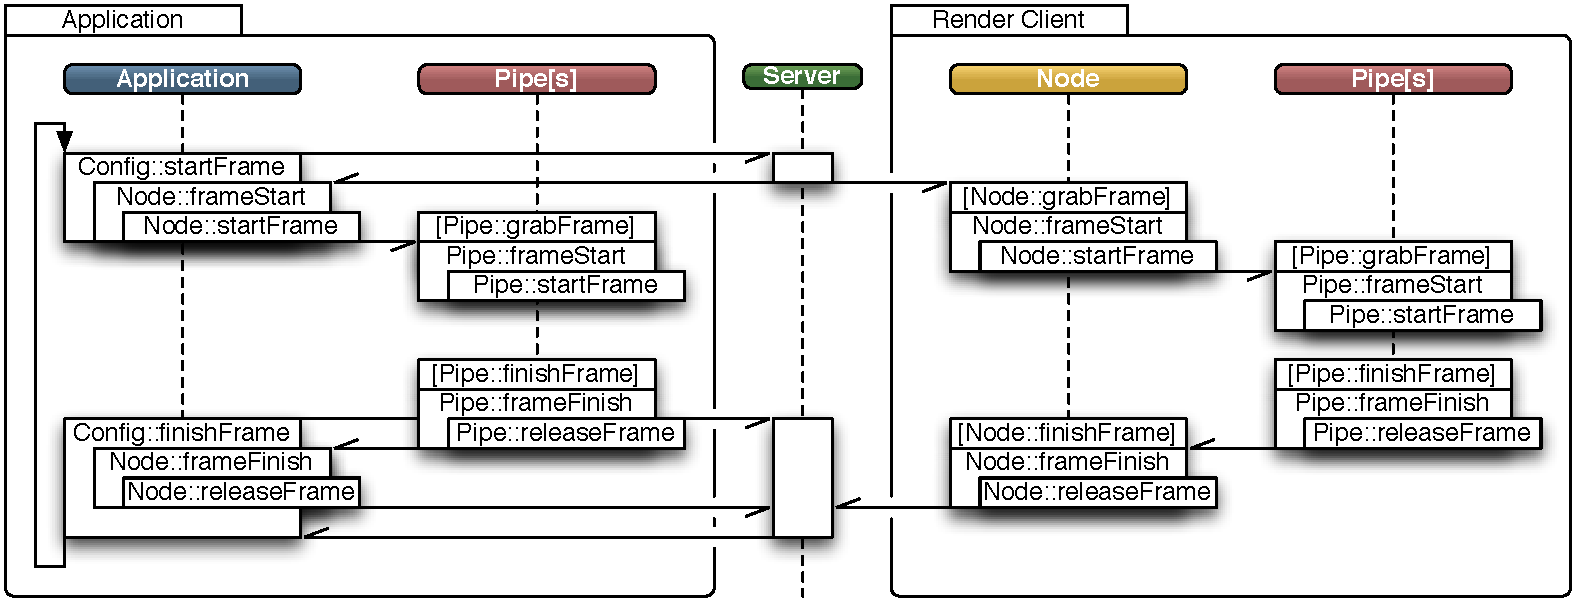
\includegraphics[width=.9\textwidth]{images/mainloop.pdf}
  {\caption{\small\label{fFrameSync}Synchronization of frame tasks}}
\end{figure}

\fig{fFrameSync} outlines the synchronization for the application, node
and pipe classes. The window and channel synchronization is similar and
omitted for simplicity. The \textsf{eqPly} example does not override
\textsf{Node::frameStart} or \textsf{frameFinish}, but it is absolutely
vital for the execution that \textsf{Node::startFrame} or
\textsf{Node::releaseFrame} are called, respectively. The default
implementation of the node task methods do take care of that.

\subsection{Pipe}

All task methods for a pipe and its children are executed in a separate
thread. This approach optimizes usage of the GPU resource, since all
tasks are executed serially and do not compete for the usage, i.e.,
context switches are minimized. Later versions of Equalizer might
introduce threaded windows to allow the parallel and independent
execution of rendering tasks on a single pipe.

\subsubsection{Initialization and Exit}

Pipe threads are not explicitely synchronized with each other, that is,
pipes might be rendering different frames at one given time. Therefore
frame-specific data has to be allocated for each pipe thread, which in
the \textsf{eqPly} example is the frame data. The frame data is a member
variable of the \textsf{eqPly::Pipe}, and is mapped to the identifier
provided by the initialization data. The initialization in
\textsf{eq::Pipe} does GPU-specific initialization, e.g., the display
connection is opened when glX/X11 is used:

{\footnotesize\begin{lstlisting}
bool Pipe::configInit( const uint32_t initID )
{
    const Node*     node        = static_cast<Node*>( getNode( ));
    const InitData& initData    = node->getInitData();
    const uint32_t  frameDataID = initData.getFrameDataID();
    eq::Config*     config      = getConfig();

    const bool mapped = config->mapObject( &_frameData, frameDataID );
    EQASSERT( mapped );

    return eq::Pipe::configInit( initID );
}
\end{lstlisting}}

The config exit is again symmetric to the config initialization. The
frame data is unmapped and GPU-specific data is de-initialized by
\textsf{eq::Config::exit}:

{\footnotesize\begin{lstlisting}
bool Pipe::configExit()
{
    eq::Config* config = getConfig();
    config->unmapObject( &_frameData );

    return eq::Pipe::configExit();
}
\end{lstlisting}}

\subsubsection{Window System}

Equalizer supports multiple window system interfaces, at the moment
glX/X11, WGL and AGL/Carbon. Some operating systems, and therefore some
Equalizer versions, support multiple window systems
concurrently\footnote{see
  \link{http://www.equalizergraphics.com/compatibility.html}}.

Each pipe might use a different window system for rendering, which is
determined before \textsf{Pipe::configInit} by
\textsf{Pipe::selectWindowSystem}. The default implementation of
\textsf{selectWindowSystem} loops over all window systems and returns
the first supported window system, determined using
\textsf{supportsWindowSystem}.

The \textsf{eqPly} examples allows selecting the window system using a
command line option. Therefore the implementation of
\textsf{selectWindowSystem} is overwritten, and returns the specified
window system, if it is supported:

{\footnotesize\begin{lstlisting}
eq::WindowSystem Pipe::selectWindowSystem() const
{
    const Node*            node     = static_cast<Node*>( getNode( ));
    const InitData&        initData = node->getInitData();
    const eq::WindowSystem ws       = initData.getWindowSystem();

    if( ws == eq::WINDOW_SYSTEM_NONE )
        return eq::Pipe::selectWindowSystem();
    if( !supportsWindowSystem( ws ))
    {
        EQWARN << "Window system " << ws 
               << " not supported, using default window system" << endl;
        return eq::Pipe::selectWindowSystem();
    }

    return ws;
}
\end{lstlisting}}%>>

Parts of the Carbon API used for window and event handling in the AGL
window system are not thread safe. The application has to call
\textsf{eq::Global::enterCarbon} before any thread-unsafe Carbon call,
and \textsf{eq::Global::leaveCarbon} afterwards. These functions should
be used only during window initialization and exit, not during
rendering. For various reasons \textsf{enterCarbon} might block up to 50
milliseconds. Carbon call in the window event handling routine
\textsf{Window::processEvent} are thread-safe, since the global carbon
lock is set in this method. Please contact the Equalizer developer
mailing list if you need to use Carbon calls on a per-frame basis.

\subsubsection{Frame Control}

All task methods for a given frame of the pipe, window and channel
entities belonging to the thread are executed in one block, starting
with \textsf{Pipe::frameStart} and finished by
\textsf{Pipe::finishFrame}. The frame start callback is therefore the
natural place to update all frame-specific data to the version belonging
to the frame. 

In \textsf{eqPly}, the version of the only frame-specific object
\textsf{FrameData} is passed as the per-frame id from
\textsf{Config::startFrame} to the frame task methods. The pipe uses
this version to update its instance of the frame data to the current
version, and then unlocks its child entities by calling
\textsf{startFrame}:

{\footnotesize\begin{lstlisting}
void Pipe::frameStart( const uint32_t frameID, const uint32_t frameNumber )
{
    _frameData.sync( frameID );
    startFrame( frameNumber );
}
\end{lstlisting}}


\subsection{Window}

The Equalizer window holds an OpenGL drawable and rendering
context. Subclassed windows should maintain all data specific to the
OpenGL context. The Equalizer window creation routines shares the OpenGL
context with the first window of the pipe, thus allowing the reuse of
OpenGL objects between all windows of one pipe, e.g., display lists and
textures.

\subsubsection{Initialization and Exit}

The initialization sequence uses multiple, overrideable task
methods. The main task method \textsf{configInit} executes a `child'
task method to create the drawable and context. The child task method
depends on the pipe's window system. The default implementations of
\textsf{configInitGLX}, \textsf{configInitWGL} or \textsf{configInitAGL}
create an on-screen window using OS-specific methods. If the OpenGL
drawable and context was created successfully, \textsf{configInit} calls
\textsf{configInitGL}, which is emant to perform the generic OpenGL
state initialization. The default implementation sets up some typical
OpenGL state, e.g., it enables the depth test.

\begin{wrapfigure}{r}{.4\textwidth}
  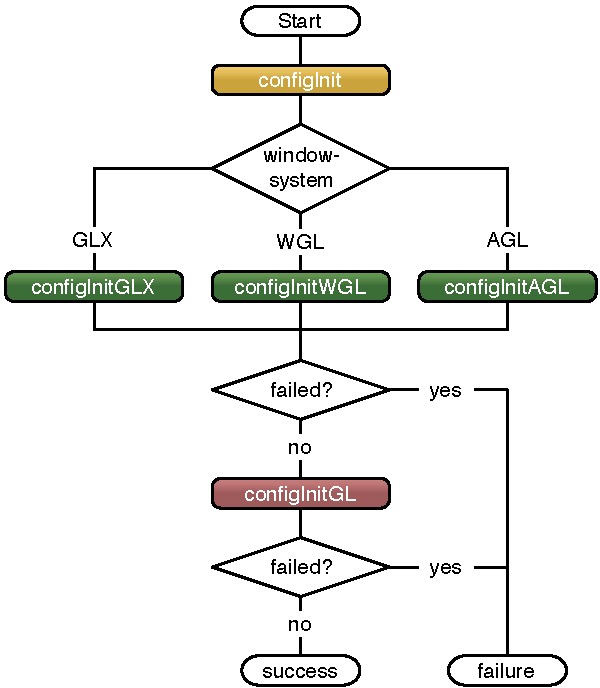
\includegraphics[width=.4\textwidth]{images/windowInit.pdf}
  {\caption{\small\label{fWindowInit}Window Initialization}}
\end{wrapfigure}
\fig{fWindowInit} shows a flow chart of the window initialization. The
colored functions are task methods and can be replaced by
application-specific implementations.

The window-system specific initialization takes into account various
attributes set in the configuration file. Attributes include the size of
various frame buffer attachments (color, alpha, depth, stencil) as well
as other framebuffer properties, such as quad-buffered stereo,
doublebuffering, fullscreen mode and window decorations. Some of the
attributes, such as stereo, doublebuffer and stencil can be set to
\textsf{eq::AUTO}, in which case the default implementation tries to use
them and gradually backs off upon failure.

The \textsf{eqPly} window initialization function first calls
\textsf{eq::Window::configInit} to use the generic window setup. If that
was successful, it initializes a state object and an overlay logo:

{\footnotesize\begin{lstlisting}
bool Window::configInit( const uint32_t initID )
{
    if( !eq::Window::configInit( initID ))
        return false;

    eq::Pipe*  pipe        = getPipe();
    Window*    firstWindow = static_cast< Window* >( pipe->getWindow( 0 ));

    EQASSERT( !_state );

    if( firstWindow == this )
    {
        _state = new VertexBufferState( getGLFunctions( ));
        _loadLogo();

        const Node*     node     = static_cast< const Node* >( getNode( ));
        const InitData& initData = node->getInitData();

        if( initData.useVBOs() )
        {
            const eq::GLFunctions* glFunctions = getGLFunctions();
            // Check if all VBO funcs available, else leave DISPLAY_LIST_MODE on
            if( glFunctions->hasGenBuffers() && glFunctions->hasBindBuffer() &&
                glFunctions->hasBufferData() && glFunctions->hasDeleteBuffers())
            {
                _state->setRenderMode( mesh::BUFFER_OBJECT_MODE );
                EQINFO << "VBO rendering enabled" << endl;
            }
            else
                EQWARN << "VBO function pointers missing, using display lists" 
                       << endl;
        }
    }
    else
    {
        _state       = firstWindow->_state;
        _logoTexture = firstWindow->_logoTexture;
        _logoSize    = firstWindow->_logoSize;
    }

    if( !_state ) // happens if first window failed to initialize
        return false;
    
    return true;
}
\end{lstlisting}}%>>

The state object is used to handle the creation of OpenGL objects in a
multipipe, multi-threaded execution environment. It uses an object
manager, which is described in detail in \sref{sObjectManager}. It is
used in conjunction with a reference pointer here, since it is
potentially `owned' by multiple windows at the same time.

The logo texture is loaded from the file system and bound to a texture
ID used later by the channel for rendering. The details of this code are
omitted here, since they are pretty straight-forward OpenGL code and not
Equalizer-specific.

The window exit deallocates all OpenGL objects when the state object is
about to be disposed. The object manager does not delete the object in
its destructor, since it does not know if an OpenGL context is still
current. In any case, \textsf{eq::Window::configExit} is called to
destroy the drawable and context:

{\footnotesize\begin{lstlisting}
bool Window::configExit()
{
    if( _state.isValid() && _state->getRefCount() == 1 )
        _state->deleteAll();

    _state = 0;
    return eq::Window::configExit();
}
\end{lstlisting}}

\subsubsection{\label{sObjectManager}Object Manager}

The object manager is --strictly speaking-- not part of the window. It
is discussed here since the \textsf{eqPly} window uses an object manager.

The state object in \textsf{eqPly} gathers all rendering state, which
includes an object manager for object state handling. This state object
can easily be replaced to use the rendering code in a stand-alone
application, e.g., for a GLUT-based renderer.

The object manager (OM) is a utility class and can be used to manage
OpenGL objects across shared contexts. Typically one OM is used for each
set of shared contexts, which normally spawns all contexts of a single
GPU\footnote{\link{http://www.equalizergraphics.com/documents/design/objectManager.html}}.

The OM is a template class. The template type is the key type, by which
objects are identified. The same key is used by all contexts to get the
OpenGL name of an object. In \textsf{eqPly}, a key of type \textsf{const
  void *} is used. The rendering code uses the address of the data item
to be rendered as the key to obtain the associated OpenGL object.

The usage of objects is reference counted. If an application releases
the objects properly, they are automatically de-allocated. It is also
possible to manually manage de-allocation of objects, which is often the
more convenient use case.

Currently handling for display lists, VBO's, textures and shaders is
implemented. For each object, the following functions are available:

\begin{description}
\item[supportsObjects()]: returns true if the usage for this particular
  type of objects is supported. For objects available in OpenGL 1.1 or
  earlier, this function is not implemented.
\item[getObject( key )]: returns the object associated with the given
  key, or FAILED. Increases the reference count of existing objects.
\item[newObject( key )]: allocates a new object for the given
  key. Returns FAILED if the object already exists or if the allocation
  failed. Sets the reference count of a newly created object to one.
\item[obtainObject( key )]: convenience function which gets or obtains
  the object associated with the given key. Returns FAILED only if the
  object allocation failed.
\item[releaseObject( key \textbar\ name )]: decreases the reference count and
  deletes the object if the reference count reaches zero.
\item[deleteObject( key \textbar\ name )]: manually deletes the object. To be
  used if reference counting is not used.
\end{description}


\subsection{Channel}

The channel is the heart of the application in that it contains the
actual rendering code. The channel is used to perform various rendering
operations for the compounds.

\subsubsection{Initialization and Exit}

During channel initialization, the near and far planes are set to
reasonable values to contain the whole model. During rendering, the near
and far planes are adjusted dynamically to the current model position:

{\footnotesize\begin{lstlisting}
bool Channel::configInit( const uint32_t initID )
{
    setNearFar( 0.1f, 10.0f );
    return true;
}
\end{lstlisting}}

\subsubsection{Rendering}

The central rendering routine is \textsf{Channel::frameDraw}. This
routine contains the application's OpenGL rendering code, which is being
rendered using the contextual information provided by Equalizer. As most
of the other task methods, \textsf{frameDraw} is called in parallel by
Equalizer on all pipe threads in the configuration. Therefore the
rendering should not write to shared data, which is the case for all
major scene graph implementations.

In \textsf{eqPly}, the OpenGL context is first set up using various
\textsf{apply} convenience methods from the base Equalizer channel
class. Each of the \textsf{apply} methods uses the corresponding
\textsf{get} method(s) and then calls the appropriate OpenGL
function(s). It is also possible to just query the values from Equalizer
using the \textsf{get} methods, and use them to set up the OpenGL state
appropriatly, for example by passing the parameters to the renderer used
by the application.

For example, the implementation for \textsf{eq::Channel::applyBuffer}
does set up the correct rendering buffer and color mask, which depends
on the current eye pass and possible anaglyphic stereo parameters:

{\footnotesize\begin{lstlisting}
void eq::Channel::applyBuffer()
{
    glReadBuffer( getReadBuffer( ));
    glDrawBuffer( getDrawBuffer( ));
    
    const ColorMask& colorMask = getDrawBufferMask();
    glColorMask( colorMask.red, colorMask.green, colorMask.blue, true );
}
\end{lstlisting}}

The contextual information has to be used in order to render the view as
expected by Equalizer. Failure to use certain information will result in
incorrect rendering for some or all configurations. The channel render
context consist of:

\begin{description}
\item[Buffer]: The OpenGL read and draw buffer as well as color mask.
  These parameters are influenced by the current eye pass, eye
  seperation and anaglyphic stereo settings.
\item[Viewport]: The two-dimensional pixel viewport restricting the
  rendering area within the channel. For correct operations, both
  \textsf{glViewport} and \textsf{glScissor} have to be used. The pixel
  viewport is influenced by the destination channel's viewport
  definition and compound viewports set for sort-first/2D decompositions.
\item[Frustum]: Frustum parameters as defined by
  \textsf{glFrustum}. Typically the frustum used to set up the OpenGL
  projection matrix. The frustum is influenced by the destination
  channel's view definition, compound viewports, head matrix and the
  current eye pass.
\item[Head Transformation]: A transformation matrix positioning the
  frustum. This is typically an identity matrix and is used for off-axis
  frustra in immersive rendering. It is normally used to set up the
  `view' part of the modelview matrix, before static light sources are
  defined.
\item[Range]: A one-dimensional range with the interval [0..1]. This
  parameter is optional and should be used by the application to render
  only the appropriate subset of its data.
\end{description}

The \textsf{frameDraw} method in \textsf{eqPly} calls the
\textsf{frameDraw} method from the parent class, the Equalizer
channel. The default \textsf{frameDraw} method uses the apply
convenience functions to setup the OpenGL state for all render context
information, with the exception of the range which will be used later
during rendering:

{\footnotesize\begin{lstlisting}
void eq::Channel::frameDraw( const uint32_t frameID )
{
    applyBuffer();
    applyViewport();
    
    glMatrixMode( GL_PROJECTION );
    glLoadIdentity();
    applyFrustum();

    glMatrixMode( GL_MODELVIEW );
    glLoadIdentity();
    applyHeadTransform();
}

void Channel::frameDraw( const uint32_t frameID )
{
    // Setup OpenGL state
    eq::Channel::frameDraw( frameID );
\end{lstlisting}}

\begin{wrapfigure}{r}{.4\textwidth}
  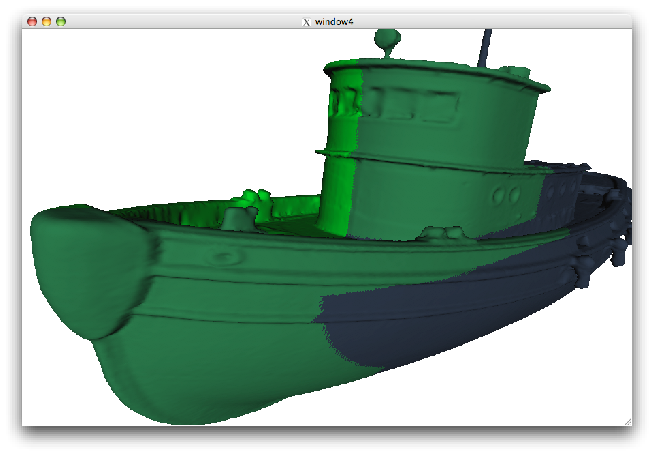
\includegraphics[width=.4\textwidth]{images/DB.pdf}
  {\caption{\small\label{fDB}Destination view of an DB compound}}
\end{wrapfigure}
After the basic view setup, a directional light is configured, and the
model is positioned using the camera parameters from the frame data. The
camera parameters are transported using the the frame data to ensure
that all channels render a given frame using the same position.

Furthermore, a white color is set in case the model does not contain
color information, or the color information is not to be used. In
sort-last rendering, \textsf{eqPly} uses a different color for each
channel to illustrate the database decomposition, as shown in
\fig{fDB}. The Equalizer channel provides a method to obtain a random,
but unique color for all channels in the configuration. This color is
determined by the server to ensure uniqueness across all channels of the
configuration:

{\footnotesize\begin{lstlisting}
    glLightfv( GL_LIGHT0, GL_POSITION, lightPosition );
    glLightfv( GL_LIGHT0, GL_AMBIENT,  lightAmbient  );
    glLightfv( GL_LIGHT0, GL_DIFFUSE,  lightDiffuse  );
    glLightfv( GL_LIGHT0, GL_SPECULAR, lightSpecular );

    glMaterialfv( GL_FRONT, GL_AMBIENT,   materialAmbient );
    glMaterialfv( GL_FRONT, GL_DIFFUSE,   materialDiffuse );
    glMaterialfv( GL_FRONT, GL_SPECULAR,  materialSpecular );
    glMateriali(  GL_FRONT, GL_SHININESS, materialShininess );

    const Pipe*      pipe      = static_cast<Pipe*>( getPipe( ));
    const FrameData& frameData = pipe->getFrameData();

    glTranslatef( frameData.data.translation.x,
                  frameData.data.translation.y,
                  frameData.data.translation.z );
    glMultMatrixf( frameData.data.rotation.ml );

    Node*            node  = (Node*)getNode();
    const Model*     model = node->getModel();
    const eq::Range& range = getRange();

    if( !range.isFull( )) // Color DB-patches
    {
        const vmml::Vector3ub color = getUniqueColor();
        glColor3ub( color.r, color.g, color.b );
    }
    else if( !frameData.data.color || (model && !model->hasColors( )) )
    {
        glColor3f( 1.0f, 1.0f, 1.0f );
    }
    
\end{lstlisting}}

Finally the model loaded by the node is rendered. If the model was not
loaded during node initialization, a quad is drawn in its place:

{\footnotesize\begin{lstlisting}
    if( model )
    {
        _drawModel( model );
    }
    else
    {
        glColor3f( 1.f, 1.f, 0.f );
        glNormal3f( 0.f, -1.f, 0.f );
        glBegin( GL_TRIANGLE_STRIP );
        glVertex3f(  .25f, 0.f,  .25f );
        glVertex3f(  .25f, 0.f, -.25f );
        glVertex3f( -.25f, 0.f,  .25f );
        glVertex3f( -.25f, 0.f, -.25f );
        glEnd();
    }
}
\end{lstlisting}}

In order to draw the model, a helper class for view frustum culling is
set up using the view frustum from Equalizer and the camera
position. The frustum helper computes the six frustum planes from the
projection and modelView matrices. During rendering, the bounding
spheres of the model are tested against these planes to determine the
visibility with the frustum. Furthermore the render state from the
window, and the database range from the channel is obtained. The render
state manages display list or VBO allocation:

{\footnotesize\begin{lstlisting}
void Channel::_drawModel( const Model* model )
{
    Window*                  window    = static_cast<Window*>( getWindow() );
    mesh::VertexBufferState& state     = window->getState();

    const Pipe*              pipe      = static_cast<Pipe*>( getPipe( ));
    const FrameData&         frameData = pipe->getFrameData();

    const eq::Range&         range     = getRange();
    vmml::FrustumCullerf     culler;

    state.setColors( frameData.data.color && 
                     range.isFull() && 
                     model->hasColors() );
    _initFrustum( culler, model->getBoundingSphere( ));

    model->beginRendering( state );
        
\end{lstlisting}}

The model data is spatially organized in an 3-dimensional
kD-tree\footnote{See also \link{http://en.wikipedia.org/wiki/Kd-tree}}
for efficient view frustum culling. When the model is loaded by
\textsf{Node::config\-Init}, it is preprocessed into the kD-tree and each
node of the tree gets a database range assigned, that is, the root node
has the range [0, 1], its left child [0, 0.5] and its right child [0.5,
1], and so on for all nodes in the tree. The preprocessed model is saved
in a binary format for accelerating subsequent use.

The rendering loop maintains a list of candidates to render, which
initially contains the root node. Each candidate of this list is tested
for full visiblity against the frustum and range, and rendered if
visible. It is dropped if it is fully invisible or fully out of
range. If it is partially visible or partially in range, the children of
the node are added to the candidate list. \fig{fRender} shows a flow
chart of the rendering algorithm, which performs efficient view frustum
and range culling.

\begin{wrapfigure}{r}{.6\textwidth}
  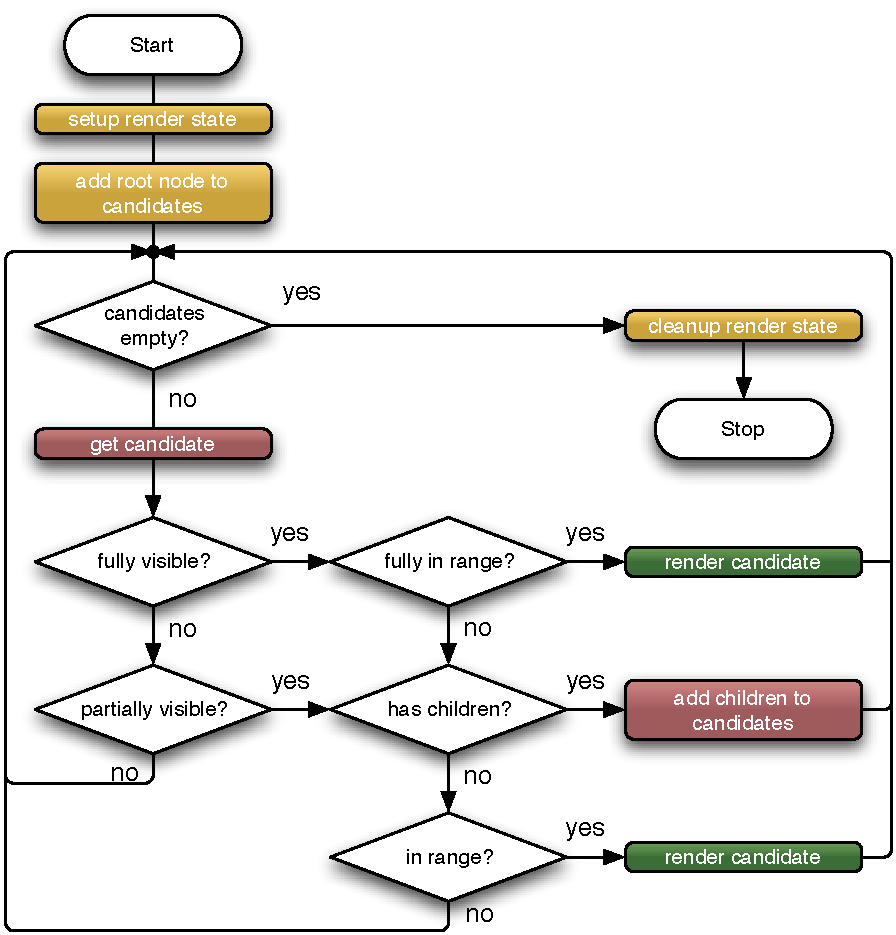
\includegraphics[width=.6\textwidth]{images/render.pdf}
  {\caption{\small\label{fRender}Main Rendering Loop}}
\end{wrapfigure}
The actual rendering uses display lists or vertex buffer objects. The
OpenGL objects are allocated using the object manager. The rendering is
done by the leaf nodes, which are small enough to store the vertex
indices in a \textsf{short} value for optimal performance with VBO's.

The leaf nodes reuse the objects stored in the object manager, or create
and set up new objects if it was not yet set up. Since one object
manager is used per thread (pipe), this allows a thread-safe sharing of
the compiled display lists or VBO's across all windows of a pipe.

The main rendering loop in \textsf{eqPly} looks like this:

{\footnotesize\begin{lstlisting}
    model->beginRendering( state );
        
    // start with root node
    vector< const VertexBufferBase* > candidates;
    candidates.push_back( model );
        
    while( !candidates.empty() )
    {
        const VertexBufferBase* treeNode = candidates.back();
        candidates.pop_back();
            
        // completely out of range check
        if( treeNode->getRange()[0] >= range.end || 
            treeNode->getRange()[1] < range.start )
            continue;
            
        // bounding sphere view frustum culling
        switch( culler.testSphere( treeNode->getBoundingSphere() ) )
        {
            case vmml::VISIBILITY_FULL:
                // if fully visible and fully in range, render it
                if( treeNode->getRange()[0] >= range.start && 
                    treeNode->getRange()[1] < range.end )
                {
                    treeNode->render( state );
                    break;
                }
                // partial range, fall through to partial visibility
            case vmml::VISIBILITY_PARTIAL:
            {
                const VertexBufferBase* left = treeNode->getLeft();
                const VertexBufferBase* right = treeNode->getRight();
            
                if( !left && !right )
                {
                    if( treeNode->getRange()[0] >= range.start )
                        treeNode->render( state );
                    // else drop, to be drawn by 'previous' channel
                }
                else
                {
                    if( left )
                        candidates.push_back( left );
                    if( right )
                        candidates.push_back( right );
                }
                break;
            }
            case vmml::VISIBILITY_NONE:
                // do nothing
                break;
        }
    }
        
    model->endRendering( state );
}
\end{lstlisting}}


\section{Advanced Features}

This section discusses some additional, important features not covered
by the previous \textsf{eqPly} section. Where possible, code examples
from the Equalizer distribution are used.


\subsection{Event Handling}

Event handling requires a lot of flexibility. On one hand, the
implementation differs slightly for each operating and window system due
to conceptual differences in the OS-specific implementation. On the
other hand, each application and widget set has its own model on how
events are to be handled. Therefore, event handling in Equalizer is
customizable in any stage of the processing, to the extreme of making it
possible to disable all event-related code in Equalizer. More
information on event handling can be found on the Equalizer
website\footnote{see
  \link{http://www.equalizergraphics.com/documents/design/eventHandling.html}}.

The default implementation provides a convenient, easily accessible
event framework, while allowing all necessary customizations. It gathers
all events in the application main thread, so that the developer only
has to implement \textsf{Config::processEvent} to update its data based
on the pre-processed, generic keyboard and mouse events. It is very easy
to use and similar to an GLUT-based implementation.


\subsubsection{Threading}

Where possible, events are received and processed by a separate per-node
event thread to allow asynchronous\footnote{with respect to the
  rendering} event handling. Currently an event thread is only used by
the X11/glX window system. WGL receives and processes the events from
the pipe threads which created the windows. AGL receives the events from
application or node main thread. Whenever the term \textbf{event thread}
is used, it refers to the thread receiving the event, i.e., a per-node
thread for glX, the pipe thread for WGL and the main thread for AGL.

\subsubsection{Initialization and Exit}

During window and pipe initialization the event handling is set up. For
both entities, \textsf{initEvent\-Handler} is called to register the
pipe or window with an event handler. This method may be overwritten to
use a custom event handler, or to not install an event handler to
disable event handling. Likewise, \textsf{exitEventHandler} is called to
de-initialize event handling.

\begin{wrapfigure}{r}{.4\textwidth}
  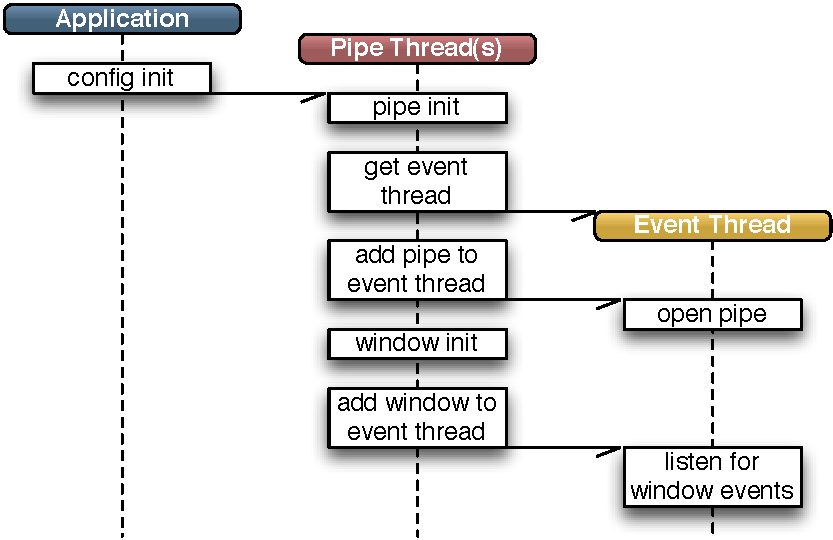
\includegraphics[width=.4\textwidth]{images/eventInit.pdf}
  {\caption{\small\label{fEventInit}Event Handling Initialization}}
\end{wrapfigure}
An event handler consists of two parts: the generic base class providing
the interface and generic functions, and the window-system-specific
part providing the actual implementation. 

Pipe event handling is only used for glX, where one \textsf{Display}
connection is created to subscribe to window events. Event handling is
initialized whenever a new, window-system-specific pipe or window handle
is set. First, \textsf{exitEventHandler} is called to de-initialize
event handling for the old handle (if set), and then
\textsf{initEvent\-Handler} is called for the new handle. AGL and glX use
an event handler singleton, whereas WGL uses one event handler per
window.

\subsubsection{Message Pump}

For the WGL and AGL window system it is required to manually receive and
dispatch (`pump') events. On WGL, this has to happen on each thread with
windows, whereas on AGL it has to happen only on the main thread. By
default, Equalizer pumps these events automatically for the application.

The methods \textsf{Client::useMessagePump} and
\textsf{Pipe::useMessagePump} can be overridden to return \textsf{false}
to disable this behaviour for their respective threads. On non-threaded
pipes, \textsf{Pipe::useMessagePump} is not called.

If the application disables message pumping in Equalizer, it has to make
sure the events are pumped externally, as it often done within external
widget sets, e.g., Trolltech's Qt.


\subsubsection{Event Data Flow}

\begin{wrapfigure}{r}{.4\textwidth}
  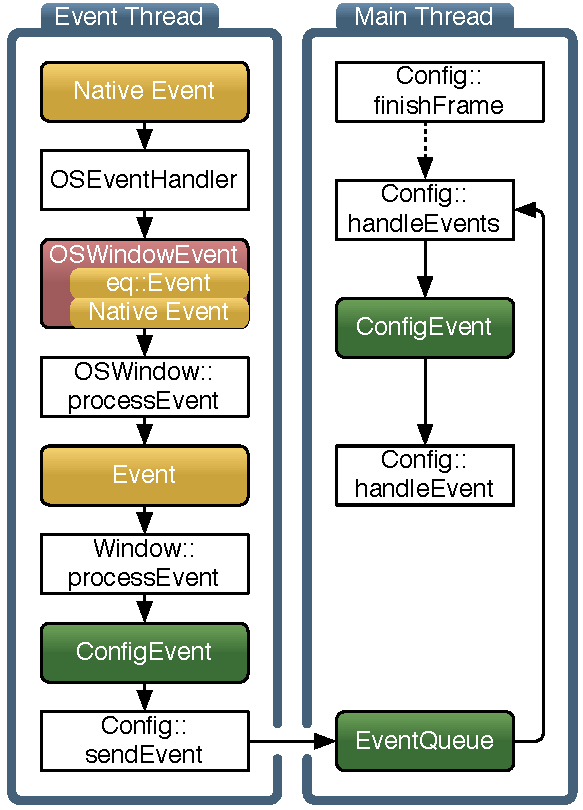
\includegraphics[width=.4\textwidth]{images/eventFilter.pdf}
  {\caption{\small\label{fEventProcessing}Event Processing}}
\end{wrapfigure}
Events are received by an event handler. The event handler finds the
\textsf{eq::Window} associated to the event. It then creates a generic
\textsf{WindowEvent}, which holds important event data in a format
independent of the window system. The original event is attached to the
generic window event.

The event handler then passes the window event to
\textsf{Window::processEvent}, which is responsible for either handling
the event locally, or for translating it into a generic
\textsf{ConfigEvent}. The config events are send to the application
thread using \textsf{Config::sendEvent}. If the event was processed, the
function has to return \textsf{true}. If \textsf{false} is returned, the
event will be passed to a previously installed, window-system-specific
event handling function. The default implementation of
\textsf{Window::processEvent} passes most events on to the application.

Events sent using \textsf{Config::sendEvent} are queued in the
application thread. After a frame has been finished,
\textsf{Config::finishFrame} calls \textsf{Config::handleEvents}. The
default implementation of this method provides non-blocking event
processing, that is, it calls \textsf{Config::handleEvent} for each
queued event. By overriding this function, event-driven execution can be
implemented.

Later Equalizer versions will introduce \textsf{Pipe::processEvent} and
\textsf{PipeEvent} to communicate pipe-specific events, e.g, resolution
changes.

\subsubsection{Custom Events in eqPixelBench}

The \textsf{eqPixelBench} example is a benchmark program to measure the
pixel transfer rates from and to the framebuffer of all channels within
a configuration. It uses custom config events to send the gathered data
to the application. It is much simpler than the \textsf{eqPly} example
since it does not provide any useful rendering or user interaction.

The rendering routine of \textsf{eqPixelBench} in
\textsf{Channel::frameDraw} loops through a number of pixel formats and
types. For each of them, it measures the time to readback and assemble a
full-channel image. The format, type, size and time is recorded in a
config event, which is sent to the application.

The \textsf{ConfigEvent} derives from the \textsf{eq::ConfigEvent}
structure and has the following definition:

{\footnotesize\begin{lstlisting}
struct ConfigEvent : public eq::ConfigEvent
{
public:
    enum Type
    {
        READBACK = eq::ConfigEvent::USER,
        ASSEMBLE
    };

    ConfigEvent()
        {
            size = sizeof( ConfigEvent );
        }

    // channel name is in user event data
    char           formatType[64];
    vmml::Vector2i area;
    float          msec;
};
\end{lstlisting}}

The \textsf{Config::sendEvent} method transmits a
\textsf{eq::ConfigEvent} or derived class to the application. The
ConfigEvent has to be a C-type structure, and its \textsf{size}
member has to be set to the full size of the event to be transmitted.
Each event has a type, by which the config processing function can
identify it. 

User-defined types start at \textsf{eq::ConfigEvent::USER}, and the
member variable \textsf{ConfigEvent::user} can be used to store
\textsf{EQ\_USER\_EVENT\_SIZE}\footnote{currently 32 bytes} bytes. In
this space, the channel's name is stored. Additional variables are used
to transport the pixel format and type, the size and the time it took
for rendering.

On the application end, \textsf{Config::handleEvent} uses the ostream
operator for the derived config event to output these events in a nicely
formatted way:

{\footnotesize\begin{lstlisting}
std::ostream& operator << ( std::ostream& os, const ConfigEvent* event );
...
bool Config::handleEvent( const eq::ConfigEvent* event )
{
    switch( event->type )
    {
        case ConfigEvent::READBACK:
        case ConfigEvent::ASSEMBLE:
            cout << static_cast< const ConfigEvent* >( event ) << endl;
            return true;

        default:
            return eq::Config::handleEvent( event );
    }
}
\end{lstlisting}}%>>


\subsection{\label{sCompositing}Image Compositing for Scalable Rendering}

Two task methods are responsible for collecting and compositing the
result image during scalable rendering, when multiple channels are
rendering for a single view. The source channels producing one or more
\textsf{outputFrame}s use \textsf{Channel::frameReadback} to read the
pixel data from the frame buffer. The channels receiving one or multiple
\textsf{inputFrame}s use \textsf{Channel::frameAssemb\-le} to assemble
the pixel data into the framebuffer. Equalizer takes care of the network
transport of frame buffer data between nodes, if needed.

Normally the programmer does not need to interfere with the image
compositing, or only at a high level, for example to order the input
frames or to optimize the readback. The following sections provide a
detailed description of the image compositing API in Equalizer.

\subsubsection{Parallel Direct Send Compositing}

In order to provide a motivation for the design of the image compositing
API, the direct send parallel compositing algorithm is introduced in this
section.

The motivation for direct send is to parallelize the costly
recomposition for database (sort-last) decomposition. With each
additional source channel, the amount of pixel data to be composited
grows linearly. When using the naive approach of compositing all frames
on the destination channel, this channel quickly becomes the bottleneck
in the system. Direct send distributes this workload evenly across all
source channels, and thereby keeps the compositing work per channel
constant.

\begin{wrapfigure}{r}{.6\textwidth}
  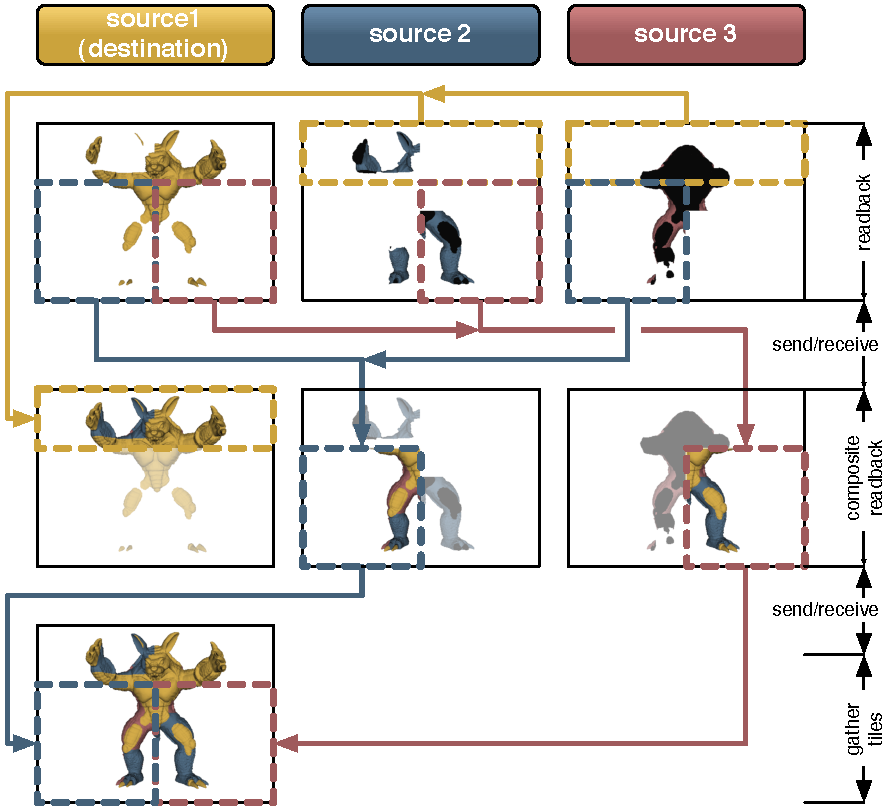
\includegraphics[width=.6\textwidth]{images/directSend.pdf}
  {\caption{\small\label{fDirectSend}Parallel Direct Send Compositing}}
\end{wrapfigure}
In direct send compositing, each rendering channel is also responsible
for the sort-last composition of one screen-space tile. He receives the
framebuffer pixels for his tile from all the other channels. The size of
one tile decreases linearly with the number of source channels, which
keeps the total amount of pixel data per channel constant.

After performing the sort-last compositing, the color information is
transferred to the destination channel, similarly to an 2D (sort-first)
compound. The amount of pixel data for this part of the compositing
pipeline also approaches a constant value, i.e., the full frame buffer.

\fig{fDirectSend} illustrates this algorithm for three channels. The
Equalizer website contains a presentation for this
algorithm\footnote{\link{http://www.equalizergraphics.com/documents/EGPGV07.pdf}}.

The following operations have to be possible in order to perform this
algorithm:
\begin{itemize}
\item Selection of frame buffer attachments: color and/or depth
\item Restricting the read back area to a part of the rendered area
\item Positioning the pixel data correctly on the receiving channels
\end{itemize}

Furthermore it should be possible for the application to implement a
read back of only the relevant region of interest, that is, the 2D area
of the framebuffer actually updated during rendering. This optimization
will be fully supported by later versions of Equalizer.

\subsubsection{Frame, Frame Data and Images}

An \textsf{eq::Frame} references an \textsf{eq::Fra\-me\-Data}. The
frame data is the object connecting output with input frames. Output and
input frames with the same name and from the same compound tree will
reference the same frame data.

The frame data is a holder for images and is used to signal the
availability of the pixel data. An \textsf{eq::Image} holds a
two-dimensional snapshot of the framebuffer and can contain color and/or
depth information.

The frame data transports the inherited range of its compound. The range
is needed to compute the assembly order of multiple input frames, e.g.,
for sorted-blend compositing in volume rendering applications.

Readback and assemble operations on frames and images are designed to be
asynchronous. They have a start and finish method for both readback and
assemble to allow the initiation and synchronization of the operation.
Currently, only synchronous readback and assembly using
\textsf{glReadPixels} and \textsf{glDrawPixels} is implemented in the
respective start method of the image.

\begin{wrapfigure}{r}{.6\textwidth}
  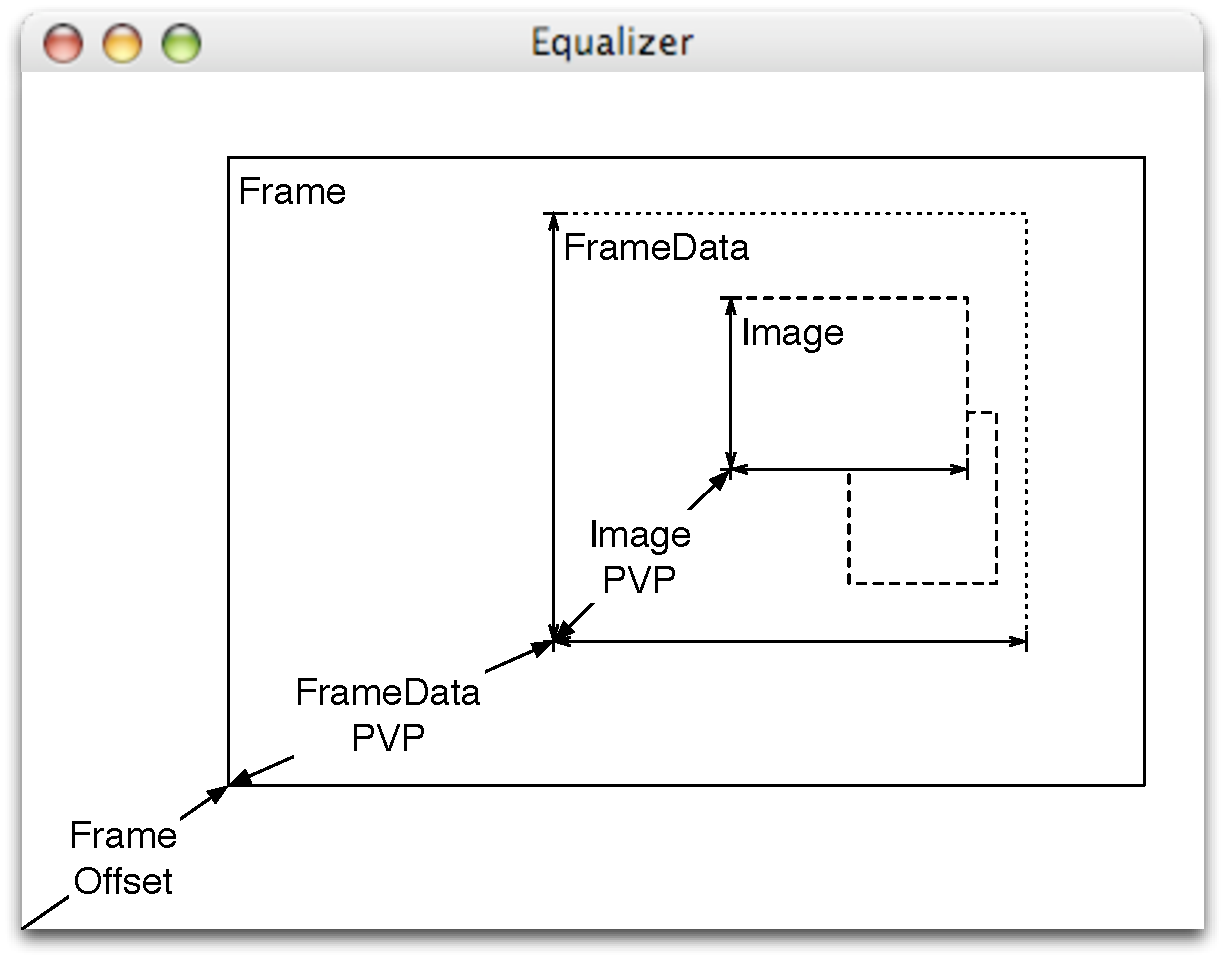
\includegraphics[width=.6\textwidth]{images/assembly.pdf}
  {\caption{\small\label{fAssembly}Hierarchy of assembly classes}}
\end{wrapfigure}
The offset of input and output frames characterizes the position of the
frame data with respect to the framebuffer, that is, the
\textbf{window's} lower-left corner. For output frames this is the
position of the channel with respect to the window.

For output frames, the frame data's pixel viewport (pvp) is the area of
the frame buffer to read back. It will transport the offset from the
source to the destination channel, that is, the frame data pvp for input
frames position the pixel data on the destination. This has the effect
that a partial framebuffer readback will end up in the same place in the
destination channels.

The image pixel viewport signifies the region of interest read
back. Currently this pvp has no offset and is as big as the frame data
pvp. Only one image will be read back.

\fig{fAssembly} illustrates the relationship between frames, frame data
and images.

\subsubsection{Custom Assembly in eVolve}

\begin{wrapfigure}{r}{.4\textwidth}
  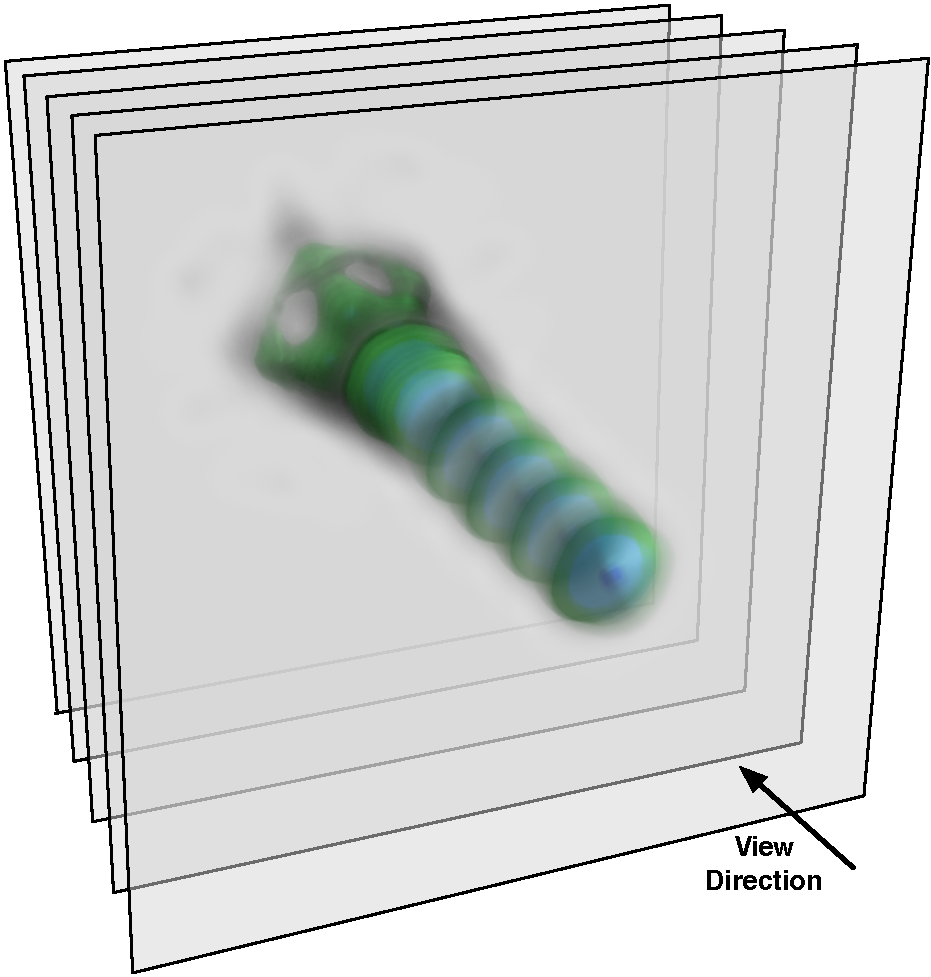
\includegraphics[width=.4\textwidth]{images/slices.pdf}
  {\caption{\small\label{fSlices}Blending Slices in 3D-Texture-based
      Volume Rendering}}
\end{wrapfigure}
The \textsf{eVolve} example is a scalable volume renderer. It uses 3D
texture-based volume rendering, where the 3D texture is intersected by
view-aligned slices. The slices are rendered back-to-front and blended
together to produce the final image, as shown in
\fig{fSlices}\footnote{Volume Data Set courtesy of: SFB-382 of the German
  Research Council (DFG)}.

When using 2D (sort-first) or stereo decompositions, no special
programming is needed to achieve good scalability, as \textsf{eVolve} is
mostly fill-limited and therefore scales nicely in this mode. 

The full power of scalable volume rendering is however in DB (sort-last)
compounds, where the full volume is divided into separate bricks. Each
of the bricks is rendered the same as in the other modes. For
recomposition, the \textsf{RGBA} frame buffer data resulting from these
render passes then has to be assembled correctly.

DB compounds have the advantage of scaling any part of the volume
rendering pipeline: texture and main memory (smaller bricks for each
channel), fill rate (less samples per channel) and IO bandwidth for
time-dependend data (less data per time step and channel).

\begin{figure}[h!t]
  \subfigure[]{\label{fBlendOrtho}
    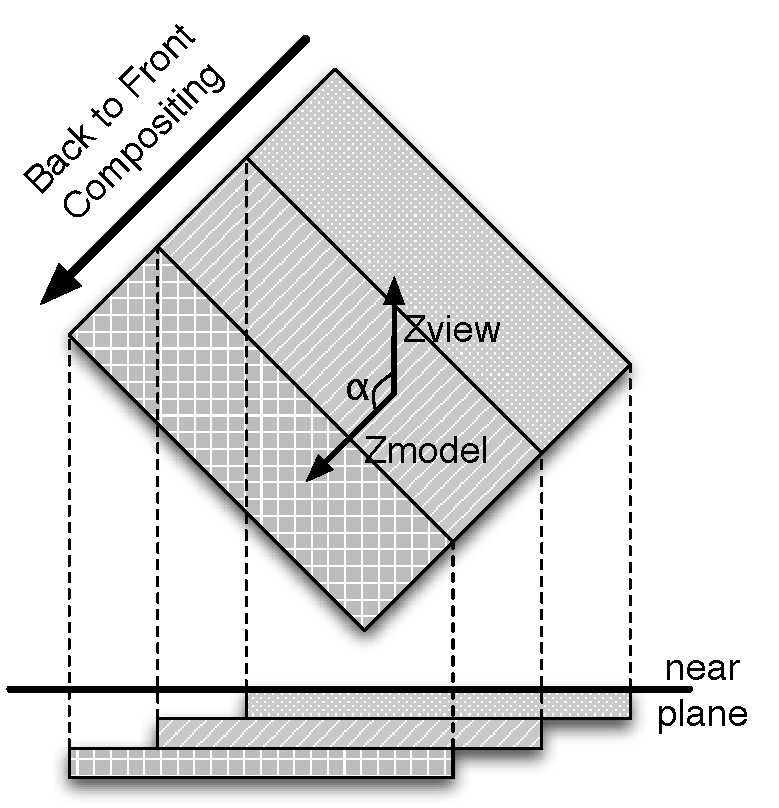
\includegraphics[width=.45\textwidth]{images/b2f_ortho.pdf}
  }\hfil
  \subfigure[]{\label{fBlendPerspective}
    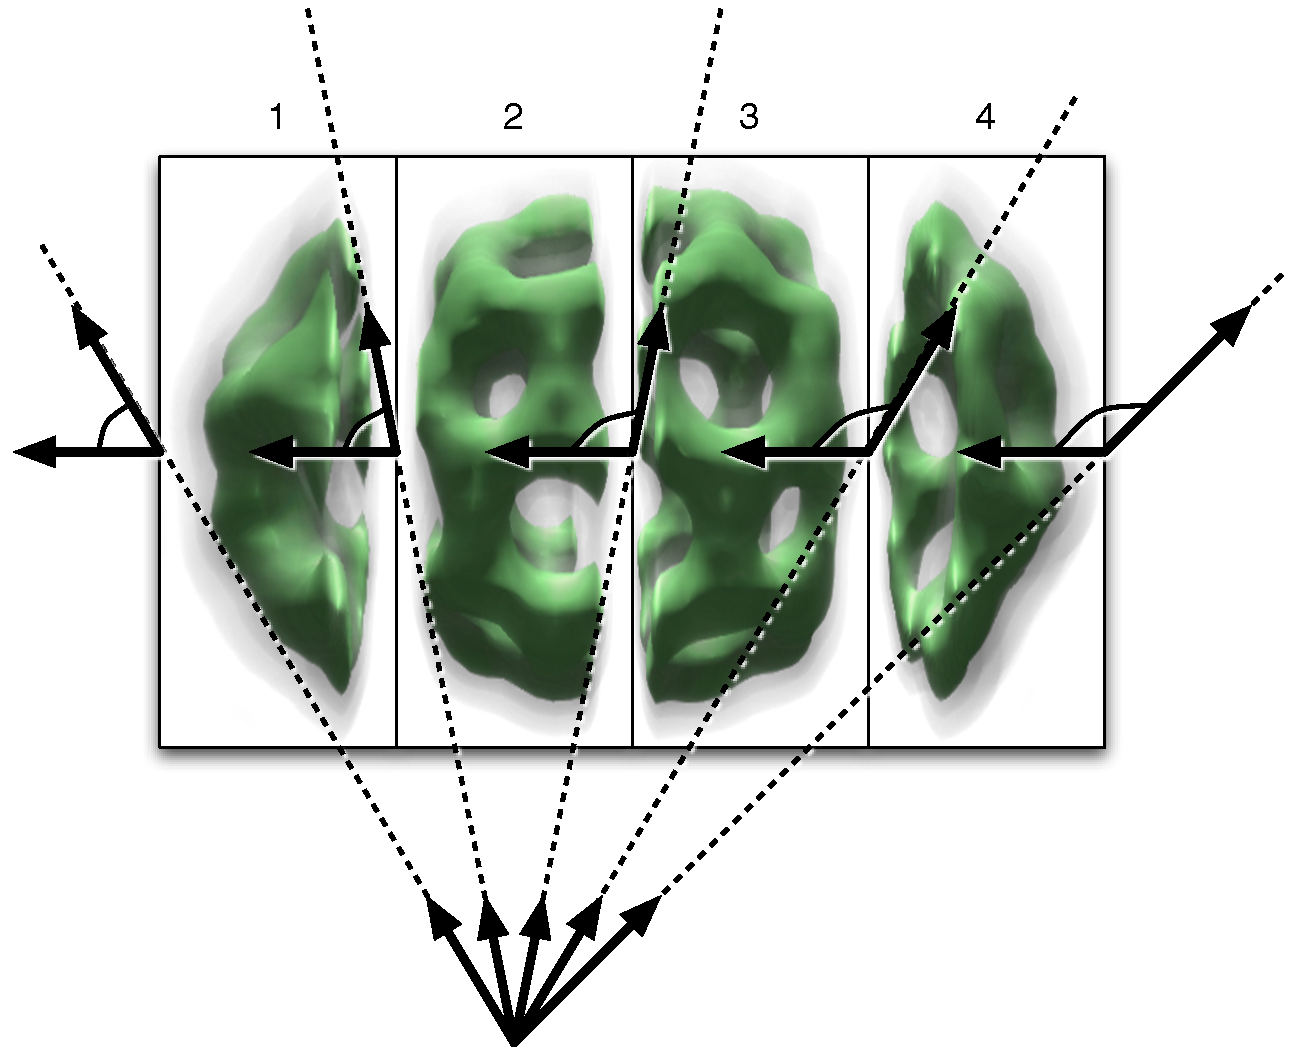
\includegraphics[width=.55\textwidth]{images/b2f_perspective.pdf}
  }%
  {\caption{\small\label{fBlend}Back-to-Front Com\-po\-siting for
      Orthogonal and Perspective View Frustra}}
\end{figure}
For recomposition, the 2D frame buffer contents are blended together to
form a seamless picture. For currect blending, the frames are ordered in
the same back-to-front order as the slices used for rendering using the
same blending parameters. Simplified, the frame buffer images are
`thick' slices which are `rendered' by writing their content to the
destination frame buffer using the correct order. 

For orthographic rendering, determining the compositing order of the
input frames is trivial. The screen-space orientation of the volume
bricks determines the order in which they have to be composited. The
bricks in \textsf{eVolve} are created by slicing the volume along one
dimension. Therefore the range of the resulting frame buffer images,
together with the sorting order, is used to arrange the frames during
compositing. \fig{fBlendOrtho} shows this composition for one view.

\begin{wrapfigure}{r}{.4\textwidth}
  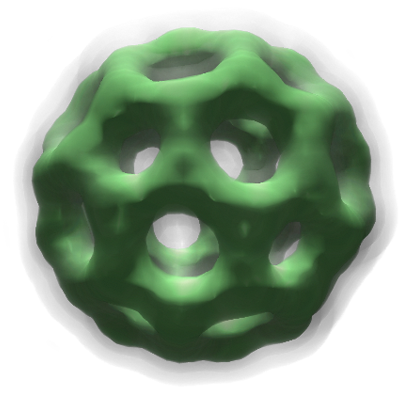
\includegraphics[width=.4\textwidth]{images/volResult.png}
  {\caption{\small\label{fVolResult}Result of \fig{fBlendPerspective}}}
\end{wrapfigure}
Finding the correct assembly order for a perspective frustra is more
complex. The perspective distortion invalidates a simple orientation
criteria like the one used for orthographic frustra. For the view and
frustum setup shown in \fig{fBlendPerspective}\footnote{Volume Data Set
  courtesy of: AVS, USA} the correct compositing order is 4-3-1-2 or
1-4-3-2.

In order to compute the assembly order, \textsf{eVolve} uses the angle
between the origin$\rightarrow$slice vector and the near plane, as shown
in \fig{fBlendPerspective}. The result image naturally looks the same as
the volume rendering would when rendered n a single channel, as shown in
\fig{fVolResult}.

The assembly algorith described in this section also works with parallel
compositing algorithms, such as direct-send.

\subsection{Head Tracking}

The \textsf{eqPly} example contains rudimentary support for head
tracking, in order to show how head tracking can be integrated with
Equalizer. Supporting a wide range of tracking devices is not within the
scope of Equalizer. Other open source and commercial implementations
cover this functionality sufficiently and can easily be integrated with
Equalizer.

\begin{figure}[h!t]
  \subfigure[]{\label{fMono}
    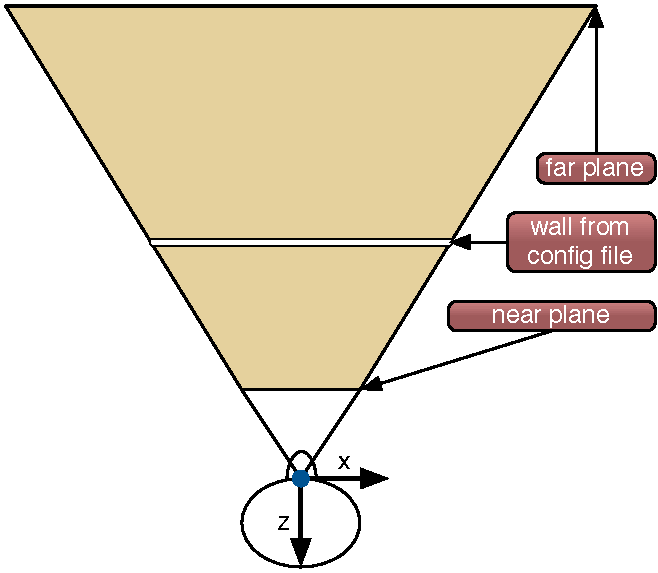
\includegraphics[width=.3\textwidth]{images/mono}}\hfil
  \subfigure[]{\label{fStereo}
    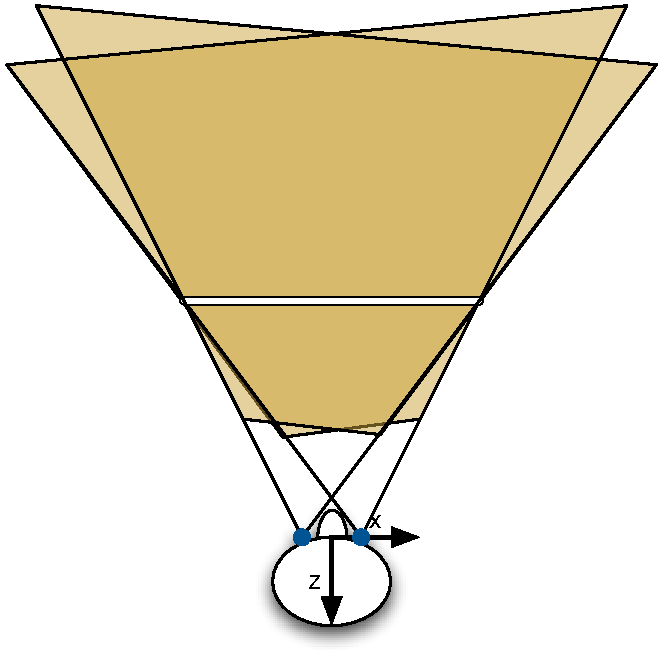
\includegraphics[width=.3\textwidth]{images/stereo}}\hfil
  \subfigure[]{\label{fTracked}
    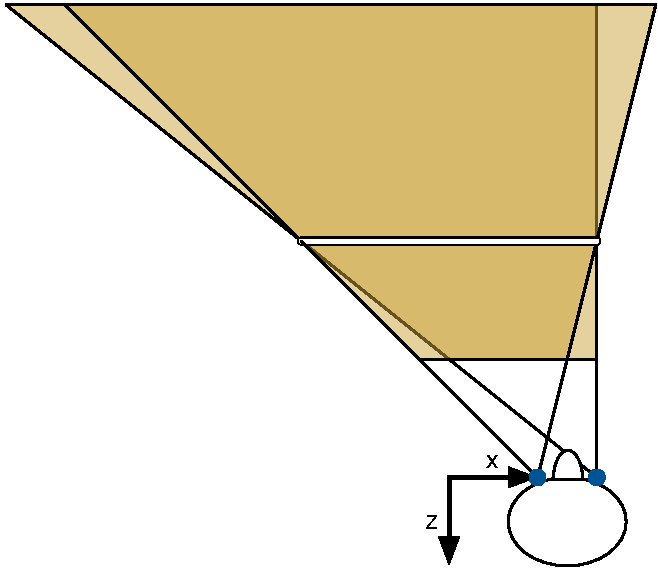
\includegraphics[width=.3\textwidth]{images/tracked}}%
  {\caption{\small\label{fImmersive}Monoscopic, Stereoscopic and Tracked
    frustra}}
\end{figure}

\fig{fMono} illustrates a monoscopic view frustum. The viewer is
positioned at the origin, and the frustum is completely symmetric. This
is the typical view frustum for non-stereoscopic applications.

In stereo rendering, the scene is rendered twice, with the two frustra
'moved' by the distance between the eyes, as shown in \fig{fStereo}.

In immersive visualization, the observer is tracked in and the view
frustra are adapted to the viewer's position and orientation, as shown
in \fig{fTracked}. The transformation origin $\rightarrow$ viewer is set by
the application using \textsf{Config::setHeadMatrix}, which is used by
the server to compute the frustra. The resulting off-axis frustra are
positioned using the channel's head transformation.

\if 0
{\footnotesize\begin{lstlisting}
\end{lstlisting}}
\fi

\end{document}
